% main.tex - Documento principale della tesi
\documentclass[12pt,a4paper,twoside,openright]{extreport}

% Pacchetti principali
\usepackage{amsmath}                            % Controllo sulle equazioni 
\usepackage{siunitx}
\usepackage{csquotes}                           % Citazioni
\usepackage{enumitem}                           % Controllo sulle enumerazioni
\usepackage[
    a4paper,
    top=2cm,bottom=2cm,
    outer=2cm,inner=2cm,
    includeheadfoot
]{geometry}                                     % Margini richiesti dall'università
\usepackage{graphicx}                           % Immagini
\usepackage{icomma}                             % Separazione decimali con virgola
\usepackage{minted}                             % Codice con colorazione sintassi
\usepackage[a-1a]{pdfx}                         % Formato PDF/A richiesto
\usepackage[output-decimal-marker={,}]{siunitx} % Unità di misura
\usepackage{subcaption}                         % Sottodidascalie
\usepackage{svg}                                % File SVG
\usepackage{float}                              % Controllo posizione immagini
\usepackage{hyperref}                           % Link ipertestuali
\usepackage{cite}                               % Citazioni bibliografiche
\usepackage[italian]{babel}                     % Lingua italiana
\selectlanguage{italian}

% Bibliografia
\usepackage[backend=bibtex,style=ieee]{biblatex}
\addbibresource{bibliografia.bib}

% Font
\usepackage{fontspec}
\setmainfont{Times New Roman}

% Impostazioni generali
\usepackage{setspace}
\onehalfspacing                                  % Interlinea 1.5 richiesto
\sloppy                                          % Evita traboccamenti di testo

% Glossario
\usepackage{glossaries}                          % Gestione glossario
\makeglossaries
\newglossaryentry{corpus}{
    name=corpus,
    description={In ambito linguistico e testuale, un corpus è un insieme strutturato e selezionato di testi raccolti secondo criteri specifici, utilizzato per l’analisi quantitativa e qualitativa di fenomeni linguistici, stilistici o discorsivi. Un corpus può essere costituito da testi scritti, trascrizioni di parlato o materiali multimediali, a seconda degli obiettivi della ricerca}
}

\newglossaryentry{bias-linguistici}{
    name=bias linguistici,
    description={Declinazioni sistematiche e non neutre nel linguaggio utilizzato per descrivere eventi, persone o fenomeni, che riflettono e talvolta rafforzano pregiudizi culturali, politici o ideologici. I bias linguistici si manifestano attraverso scelte lessicali, sintattiche o stilistiche che possono influenzare la percezione e l'interpretazione da parte del destinatario}
}

\newglossaryentry{survey-internazionali}{
    name=survey-internazionali,
    description={Indagini statistiche condotte su scala globale o sovranazionale, finalizzate alla raccolta sistematica di dati comparabili tra differenti paesi o aree geografiche. Tali rilevazioni utilizzano metodologie standardizzate per analizzare opinioni, atteggiamenti, comportamenti o caratteristiche socio-demografiche, consentendo confronti empiricamente fondati a livello internazionale}
}

\newglossaryentry{framing}{
    name=framing,
    description={Il framing (o effetto framing) si riferisce al modo in cui una situazione o un'informazione sono presentati, e come questo influenza la percezione e l'interpretazione che ne fa il pubblico. In sostanza, è come se un'immagine fosse incorniciata: la cornice, ovvero il modo in cui l'immagine è presentata, può cambiare significativamente la nostra percezione della stessa, anche se il contenuto rimane invariato.}
}

\newglossaryentry{agenda-setting}{
    name=agenda setting,
    description={L'agenda-setting, nel campo della comunicazione, è una teoria che spiega come i media siano in grado di influenzare la percezione del pubblico riguardo agli argomenti più significativi. Essi riescono a "definire l'agenda" del dibattito pubblico attraverso la selezione delle notizie ritenute rilevanti e attribuendo a queste un determinato livello di importanza.}
}

\newglossaryentry{frame-interpretativi}{
    name=frame-interpretativi,
    description={I frame interpretativi rappresentano strumenti che condizionano la nostra comprensione e interpretazione del mondo. Essi funzionano analogamente a "cornici" concettuali, facilitando la selezione, l'organizzazione e l'attribuzione di significato agli eventi e alle informazioni che assimilamo, modellando in tal modo la nostra percezione complessiva della realtà.}
}                      % Caricamento definizioni glossario

% Dati frontespizio
\title{La politicizzazione del linguaggio giornalistico: analisi di bias e strategie narrative}

\begin{document}
    \pagenumbering{roman}
    \pagestyle{empty}
    
    \begin{titlepage}
    % solo il frontespizio deve essere simmetrico rispetto ai margini interno ed esterno
    \newgeometry{hmargin=2.5cm,vmargin=2cm}
        \begin{figure}
            \centering
            \begin{subfigure}[b]{0.4\textwidth}
                
\includegraphics[width=\textwidth]{Immagini/logo_unipd}
            \end{subfigure}
            \hfill
            \begin{subfigure}[b]{0.3\textwidth}
                
\includegraphics[width=\textwidth]{Immagini/logo.png}
            \end{subfigure}
        \end{figure}
    
        \vspace*{\stretch{0.5}}
    
        \begin{center}
            \makeatletter % serve per poter usare \@...

            % NOTA: il Times New Roman non supporta il maiuscoletto.
            %\textsc{DIPARTIMENTO DI INGEGNERIA DELL'INFORMAZIONE}\\
            %\vspace*{\stretch{0.1}}
            %\textsc{CORSO DI LAUREA IN INGEGNERIA ...}
    
            \vspace*{\stretch{0.5}}
            \LARGE
            \textbf{\@title}
    
            \vspace*{\stretch{1}}
            \normalsize
            \begin{tabular*}{\textwidth}{l @{\extracolsep{\fill}} r}
                \textbf{Relatore} & \textbf{Autori} \\
                Prof. Andrea Sciandra & 
                \begin{tabular}[t]{@{}r@{}}
                    Alvise Garberino \\
                    Tommaso Orlandini \\
                    Jacopo Falasco
                \end{tabular} \\
            \end{tabular*}
    
            \vspace*{\stretch{2}}
            \textsc{ANNO ACCADEMICO 2024-2025} \\
            \vspace*{\stretch{0.1}}
            %Data di laurea \@date
        
            \makeatother % serve dopo \makeatletter
        \end{center}
    \restoregeometry
\end{titlepage}

    \cleardoublepage
    
    \vspace*{\stretch{1}}
\begin{flushright}
    \textit{Apes. Together. Strong.}
\end{flushright}
\vspace{\stretch{4}}
    \cleardoublepage
    
    \pagestyle{plain}
    
    \chapter*{Sommario}
    La ricerca si basa su una domanda a cui non perviene, o quasi mai, una risposta certa: "Le testate giornalistiche caratterizzate da posizionamenti politici differenti confezionano, anche in assenza di esplicite manipolazioni, narrazioni alternative di uno stesso fatto attraverso scelte linguistiche e strategie di \gls{framing}?". A tal scopo, si propone un’analisi comparativa di un \gls{corpus} di articoli riguardanti l’attuale presidente degli Stati Uniti Donald Trump. 
    I testi saranno in primo luogo classificati in base al contesto tematico, quindi sottoposti ad un’analisi testuale focalizzata sull’emergere di \gls{bias-linguistici}, meccanismi di \gls{agenda-setting} e processi di costruzione narrativa; infine, saranno discussi i risultati quantitativi e qualitativi ottenuti.
    \cleardoublepage
    
    \pagenumbering{arabic}

    \listoftables
    \cleardoublepage

    \listoffigures
    \cleardoublepage
    
    \tableofcontents
    \chapter{Orientamenti politici delle principali testate giornalistiche mondiali}
\label{chap:orientamenti_press}

\section{Introduzione}
In questo capitolo vengono analizzati gli orientamenti politici delle principali testate giornalistiche mondiali. Il quadro editoriale internazionale si distingue in diverse macro-aree — neutrali, centro-sinistra, centro, centro-destra, e cattolico-centrista — ottenute attraverso esercitazioni universitarie, analisi testuali quantitative e \gls{survey-internazionali}.

\section{Classificazione delle testate}
Di seguito la classificazione delle principali testate mondiali in base al loro orientamento politico:

\begin{table}[h]
  \centering
  \begin{tabular}{|p{5cm}|p{10cm}|}
    \hline
    \textbf{Orientamento politico} & \textbf{Testate} \\
    \hline
    Neutrali / Indipendenti & The Guardian \cite{theguardian}, BBC News \cite{bbcnews}, Reuters \cite{reuters}, Al Jazeera \cite{aljazeera}, The New York Times \cite{thenewyorktimes}, Dawn \cite{dawn} \\
    \hline
    Centro-sinistra / Progressisti & The Washington Post \cite{thewashingtonpost}, Le Monde \cite{lemonde}, La Repubblica \cite{larepubblica}, CNN \cite{cnn}, Folha de S.Paulo \cite{folhadespaulo}, The Hindu \cite{thehindu}, Globe and Mail \cite{globeandmail}, Financial Times \cite{financialtimes}, El País \cite{elpais}, Der Spiegel \cite{derspiegel}, Süddeutsche Zeitung \cite{suddeutschezeitung}, China Daily \cite{chinadaily}, Asahi Shimbun \cite{asahishimbun} \\
    \hline
    Centro-destra / Conservatori & Corriere della Sera \cite{corrieredellasera}, The Straits Times \cite{thestraitstimes}, Bloomberg News \cite{bloombergnews}, Clarín \cite{clarín}, The Korea Times \cite{thekoreatimes}, The Wall Street Journal \cite{thewallstreetjournal} \\
    \hline
  \end{tabular}
  \caption{Classificazione delle testate giornalistiche mondiali per orientamento politico.}
  \label{tab:classificazione_testate}
\end{table}

\begin{figure}
    \centering
    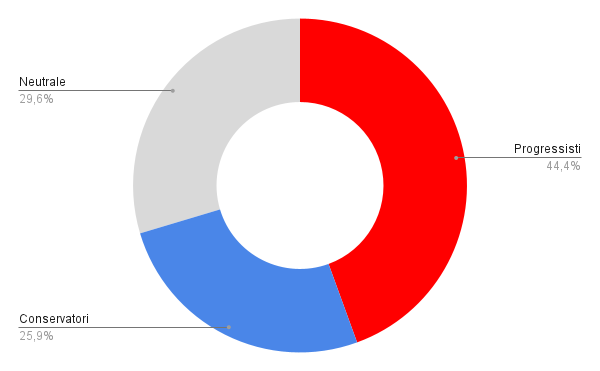
\includegraphics[width=0.75\linewidth]{Immagini/Classificazione delle Testate.png}
    \caption{Suddivisione delle testate giornalistiche utilizzate per l'analisi}
    \label{fig:enter-label}
\end{figure}

\section{Metodologia di classificazione}
Il metodo utilizzato per la classificazione delle testate giornalistiche oggetto della nostra analisi si articola in tre principali fasi. In primo luogo, è stato condotto uno studio della storia di ciascuna testata, in modo tale da comprenderne l’evoluzione editoriale, le linee guida ideologiche nel tempo, ed il contesto socio-politico in cui si è sviluppata. Successivamente, è stata effettuata una ricerca online finalizzata alla raccolta di informazioni aggiornate e pertinenti per ottenere un quadro il più possibile completo ed obiettivo. Infine, tale materiale è stato integrato con una valutazione personale elaborata a partire dalle nostre osservazioni critiche, esperienze dirette di lettura e riflessioni maturate nel corso del progetto. \\ 
Questo approccio, pur riconoscendo una componente soggettiva, mira ad offrire una classificazione ragionata e consapevole, fondata su una pluralità di prospettive e su un'analisi documentata.

    \chapter{La politicizzazione del linguaggio giornalistico}

La relazione tra giornalismo e politica è estremamente complessa, un continuo equilibrio tra collaborazione e conflitto, in quanto i politici necessitano dei media per la divulgazione delle loro azioni, ma volendone controllare il racconto. D'altra parte, i giornalisti, seppur dipendendo da tali fonti politiche, desiderano indipendenza e libertà di espressione critica \cite{giornalismo&politica}. Secondo Gianpietro Mazzoleni \cite{gpMazzoleni}, i media svolgono tre funzioni principali: informare, interpretare e persuadere.\
Le prime due sono a "disposizione degli utenti": i giornalisti rappresentano la popolazione svolgendo la funzione di mediatori tra la politica e i cittadini, offrendo un'informazione oggettiva e interpretando le notizie. La terza funzione – quella persuasiva – invece solleva interrogativi etici e politici, poiché rischia di trasformare i media in strumenti di influenza ideologica piuttosto che garanti di un'informazione libera ed equilibrata. \\
Uno dei principali problemi in questo contesto riguarda la stretta relazione sociale tra giornalisti e politici. Fabio Martini \cite{fMartini} sottolinea come i giornalisti politici vivano immersi nello stesso ambiente dei rappresentanti della politica: frequentano gli stessi ristoranti, partecipano agli stessi circoli sociali e, in molti casi, i loro figli frequentano le medesime scuole. Questa vicinanza rischia di minare l’indipendenza del racconto giornalistico, creando dinamiche di complicità, autocensura o persino collusione tra chi descrive la politica e chi la pratica. \\
Martini mette in luce come simili meccanismi relazionali emergano anche in altri ambiti professionali: tra giornalisti giudiziari e magistrati, protagonisti del mondo dello spettacolo e registi, oppure tra giornalisti economici e imprenditori. Tuttavia, è soprattutto nel rapporto tra stampa politica e classe dirigente che queste connessioni risultano più delicate e potenzialmente dannose per la trasparenza del sistema democratico. In questo scenario, il linguaggio giornalistico tende ad essere influenzato dalla politicizzazione, con effetti negativi sulla neutralità del discorso. Questo fenomeno favorisce la creazione di narrazioni orientate agli interessi delle élite politiche coinvolte. \\
La politicizzazione non si limita alla scelta dei toni e dei termini, ma si estende anche alla selezione delle informazioni, al modo in cui gli eventi vengono inquadrati (\gls{framing}) e alla definizione delle priorità nell’agenda mediatica. Questi processi contribuiscono alla costruzione di una realtà politica mediata dai mezzi di comunicazione, spesso distante dalla sua dimensione oggettiva. \\

\section{Definizioni ed Implicazioni}
Per analizzare in modo approfondito la questione relativa alla politicizzazione del linguaggio giornalistico, è indispensabile definire con precisione il significato di questa espressione. La politicizzazione può essere descritta come il processo mediante il quale il linguaggio e le pratiche del giornalismo subiscono un'influenza diretta da logiche, interessi o retoriche tipiche del discorso politico, arrivando così a perdere, parzialmente o totalmente, la loro originaria funzione di mediazione neutrale e oggettiva dell'informazione. \\
Questo fenomeno si manifesta non solo attraverso l’adozione di un lessico orientato ideologicamente, ma anche nelle modalità di selezione delle fonti, nella strutturazione gerarchica delle notizie, nei meccanismi di inquadramento narrativo (\gls{framing}) e nelle strategie volte a determinare le priorità dell’agenda informativa (\gls{agenda-setting}). In una simile prospettiva, il giornalismo rischia di mutare la propria natura trasformandosi in un mezzo di propaganda, abdicando al suo ruolo critico e di servizio pubblico per favorire narrazioni funzionali ai detentori del potere. \\
Un’informazione politicizzata contribuisce alla polarizzazione dell’opinione pubblica, all’irrigidimento delle divisioni ideologiche ed alla crescente sfiducia nei confronti dei mezzi di comunicazione. Inoltre, essa compromette il principio della libertà di stampa, subordinando la pratica giornalistica ad interessi esterni. \\
Sul piano etico, la politicizzazione richiede una riflessione approfondita sul ruolo del giornalista come attore sociale responsabile. Qualora il linguaggio utilizzato da tali professionisti risulti piegato alle logiche del potere, emergono interrogativi cruciali riguardanti la veridicità, l’imparzialità e la responsabilità civica della comunicazione giornalistica. \\
Da una prospettiva sociologica, è inoltre essenziale esaminare in che modo la politicizzazione influenzi la percezione collettiva della realtà politica. I mezzi di comunicazione non si limitano infatti a trasmettere i fatti: essi li selezionano, li interpretano e li rappresentano secondo schemi narrativi che partecipano attivamente alla costruzione di un determinato immaginario politico. \\
Pertanto, la politicizzazione del linguaggio giornalistico non si configura soltanto come una problematica interna alla professione, bensì come un elemento che contribuisce in maniera determinante a plasmare il contesto politico e culturale di una società.

\section{Il ruolo della retorica e della semantica}
Nel processo di politicizzazione del linguaggio giornalistico, la retorica e la semantica rivestono un ruolo fondamentale, si configurano come strumenti chiave nella costruzione di una rappresentazione orientata della realtà politica. Attraverso approfondite scelte lessicali, strutture narrative definite e l'utilizzo di figure retoriche, i media contribuiscono non solo a descrivere, ma anche a plasmare l'immagine che il pubblico si forma degli eventi. \\
La retorica, considerata "l'arte di persuadere per mezzo del linguaggio", viene utilizzata strategicamente per influenzare l'opinione pubblica sia in maniera esplicita che implicita. Definire, ad esempio, una manifestazione come “protesta pacifica” anziché “rivolta violenta” non rappresenta una semplice variazione stilistica, ma costituisce un atto semantico e politico che contribuisce a modellare la percezione dei fatti da parte del pubblico. \\
La dimensione semantica si manifesta soprattutto nella selezione del vocabolario e nella costruzione dei concetti. Parole come riforma, tagli, sicurezza, popolo, élite o emergenza non possiedono neutralità oggettiva, veicolano valori e orientamenti ideologici sottesi che riflettono la prospettiva dell’autore ed, al contempo, influenzano la possibile interpretazione. In tal modo, il linguaggio giornalistico gioca un ruolo estremamente cruciale nella normalizzazione di determinati punti di vista, presentando come inevitabili o necessarie scelte politiche che potrebbero essere soggette a maggiore scrutinio critico. \\
Un aspetto particolarmente rilevante di questa dinamica è la funzione performativa del linguaggio. I media non si limitano alla semplice descrizione degli eventi; al contrario, partecipano attivamente alla costruzione della realtà attraverso un uso, teoricamente, consapevole e strategico delle parole. La selezione di termini e di formule espressive genera effetti cognitivi ed emotivi sul pubblico, il che solleva interrogativi in merito alla responsabilità etica del giornalista. \\
La retorica giornalistica si rivela cruciale nella costruzione di \gls{frame-interpretativi} che orientano la comprensione collettiva dei fenomeni politici. Raccontare crisi, conflitti, eroi o nemici secondo schemi narrativi ricorrenti semplifica la complessità degli eventi e facilita la mobilitazione emotiva dell'audience. Pertanto, la semantica e la retorica si configurano come strumenti essenziali nel processo di politicizzazione del linguaggio mediatico, con un impatto profondo sia sulla percezione della realtà che sul discorso pubblico complessivo. \\
    \chapter{L’attore principale: Donald J. Trump}

\section{Profilo biografico e politico}

Donald John Trump nasce il 14 giugno 1946 a New York, figlio di Fred Trump, imprenditore immobiliare, e Mary Anne MacLeod, immigrata scozzese. Cresciuto nel Queens, frequenta la New York Military Academy e si laurea in economia presso la Wharton School dell’Università della Pennsylvania nel 1968. Dopo gli studi, entra nell’azienda di famiglia, la Trump Organization, espandendo le attività immobiliari in progetti di grande visibilità come la Trump Tower a Manhattan, hotel, casinò e campi da golf, consolidando la sua immagine di imprenditore di successo \cite{blair2001}. \\
Negli anni Ottanta e Novanta, Trump diventa una figura pubblica nota non solo per le sue attività imprenditoriali, ma anche per il suo stile di vita sfarzoso e la presenza costante nei media. La sua popolarità cresce ulteriormente grazie al reality show \emph{The Apprentice}, che lo trasforma in un personaggio televisivo di rilievo nazionale \cite{mcintosh2016}. \\
L’ingresso formale in politica avviene nel 2015, quando annuncia la candidatura alle primarie repubblicane per le elezioni presidenziali del 2016. La sua campagna si distingue per un linguaggio diretto, spesso provocatorio, e per l’uso innovativo dei social media, in particolare Twitter, come strumento di comunicazione politica \cite{ott2017}. I temi centrali della sua piattaforma includono il rafforzamento dei confini, la revisione degli accordi commerciali, la riduzione delle tasse e una politica estera improntata all’“America First”. Nonostante lo scetticismo iniziale, Trump vince le primarie e, nel novembre 2016, viene eletto 45º Presidente degli Stati Uniti, sovrastando Hillary Clinton. \\
Il suo mandato (2017–2021) è segnato da una forte polarizzazione politica e sociale, da una comunicazione fuori dagli schemi tradizionali e da decisioni controverse sia in politica interna che estera. Tra le iniziative più rilevanti si ricordano la riforma fiscale del 2017, la nomina di tre giudici alla Corte Suprema, il ritiro da accordi internazionali, come il trattato di Parigi sul clima e l’accordo sul nucleare iraniano, e la gestione della pandemia di COVID-19 \cite{baker2020}. \\
Dopo la sconfitta alle elezioni del 2020 contro Joe Biden, Trump ha continuato a esercitare una forte influenza sul Partito Repubblicano e sull’elettorato conservatore, alimentando teorie di frode elettorale e mantenendo un ruolo centrale nel dibattito politico statunitense \cite{graham2021}. La sua figura è rimasta estremamente divisiva, rappresentando per alcuni la difesa dei valori tradizionali americani e, per altri, un simbolo di populismo e attacco alle istituzioni democratiche. \\ 
Nel 2024 si è nuovamente candidato alla presidenza degli Stati Uniti affrontando una campagna elettorale caratterizzata da una retorica ancora più estrema e da un coinvolgimento senza precedenti dei suoi sostenitori \cite{nyt2024, bbc2024}. Nonostante le numerose controversie e le sfide giudiziarie è riuscito a riconquistare la leadership del Partito Repubblicano e ad imporsi nelle elezioni presidenziali, diventando così il 47º presidente degli Stati Uniti. La sua vittoria ha segnato un evento storico, rappresentando il ritorno alla Casa Bianca di un ex presidente dopo una sconfitta elettorale, e ha ulteriormente accentuato le divisioni politiche e sociali all'interno del Paese. \\
Il secondo mandato di Trump si apre in un contesto di forte tensione, con l’attenzione dei media e dell’opinione pubblica concentrata sulle sue prime decisioni e sulle possibili conseguenze per la politica interna ed estera degli Stati Uniti.\\

\section{Centralità mediatica e polarizzazione}

La centralità mediatica di Donald Trump, già evidente durante la sua prima presidenza, ha raggiunto nuovi livelli in occasione della campagna elettorale e della vittoria alle elezioni del 2024 \cite{lse2024}. Trump ha saputo sfruttare un ecosistema mediatico sempre più frammentato, caratterizzato dalla presenza di media tradizionali, piattaforme digitali, social network e, in misura crescente, podcast e canali di informazione alternativi. Questa frammentazione ha contribuito a rafforzare la polarizzazione del discorso pubblico, creando ``bolle informative'' in cui le narrazioni su Trump e sui suoi avversari risultano spesso inconciliabili \cite{pew2024}. Durante la campagna del 2024, Trump ha puntato in modo strategico su media non convenzionali, come podcast e piattaforme di streaming, raggiungendo segmenti di pubblico tradizionalmente meno coinvolti dalla politica, in particolare giovani uomini e gruppi sociali ``disillusi'' dai media mainstream. La sua presenza su podcast di grande seguito, come ``The Joe Rogan Experience'', ha permesso di bypassare i filtri giornalistici tradizionali e di consolidare un rapporto diretto e personale con l’elettorato. Questa strategia ha contribuito a un aumento significativo del consenso tra giovani e minoranze, pur restando la base elettorale di Trump prevalentemente composta da elettori bianchi \cite{newsweek2024}. La copertura mediatica della vittoria di Trump nelle ultime elezioni ha evidenziato una profonda spaccatura tra le narrazioni delle testate conservatrici e quelle progressiste. I media di destra hanno celebrato il ritorno di Trump come una rivincita contro l’establishment e i media tradizionali, mentre le testate progressiste hanno sottolineato i rischi per la democrazia e la crescente disinformazione. Questa dicotomia si riflette anche nella fiducia del pubblico nei confronti dei media: secondo recenti sondaggi, la fiducia nelle testate tradizionali ha raggiunto livelli storicamente bassi, con una crescente parte della popolazione che si informa esclusivamente tramite fonti alternative o social media \cite{pew2024}. \\
Un altro elemento centrale della polarizzazione è la tendenza dei media a enfatizzare il ruolo di specifici gruppi demografici nel successo elettorale di Trump, spesso attribuendo la vittoria a presunti ``spostamenti'' di voto tra minoranze etniche. Tuttavia, analisi più approfondite mostrano che la coalizione elettorale di Trump rimane prevalentemente bianca, e che la narrazione mediatica rischia di semplificare eccessivamente dinamiche sociali complesse, alimentando ulteriori divisioni \cite{georgetown2025}. \\
In sintesi, la rielezione di Donald Trump nel 2024 ha rappresentato non solo un evento politico di portata storica, ma anche un caso emblematico di come la centralità mediatica e la polarizzazione informativa possano influenzare profondamente la percezione pubblica e il dibattito democratico. L’analisi delle narrazioni giornalistiche relative agli eventi della sua campagna e presidenza offre uno spaccato significativo delle dinamiche di potere, fiducia e conflitto che caratterizzano il sistema mediatico contemporaneo \cite{faris2017}.
    \chapter{Metodologia dell’analisi}

\section{Selezione degli eventi analizzati}
Per analizzare come il linguaggio giornalistico possa essere influenzato dalla politica, il nostro gruppo ha scelto sei momenti significativi legati ad attività pubbliche e politiche del neo eletto presidente degli Stati Uniti d'America Donald Trump tra il 2024 e il 2025.\\
Si tratta di eventi estremamente differenti tra loro, dal comizio elettorale di Indianola, in Iowa, al World Economic Forum di Davos, tutti però accomunati da una forte visibilità, sia a livello nazionale che internazionale. \\
La scelta è ricaduta su questi episodi non solo per la loro posizione temporale, ma anche per la varietà dei temi trattati: immigrazione, politica energetica, sicurezza nazionale, economia e relazioni internazionali. \\
Ogni discorso ci ha offerto uno spunto utile per comprendere come il modo di raccontare i fatti possa cambiare a seconda della linea editoriale del giornale. \\
È necessario sottolineare che i discorsi analizzati sono stati tenuti in fasi cruciali del percorso politico di Trump: durante le primarie, l’accettazione della candidatura, successivo alla vittoria elettorale, all’insediamento ed infine in un importante evento internazionale durante il quale ha rilanciato la sua agenda. \\
Questa varietà, sia nei tempi sia nei contenuti, ci ha permesso di raccogliere un campione estremamente ampio e necessario per evidenziare tendenze ricorrenti e differenze di stile tra le varie aree ideologiche del panorama dell’informazione.\\

\section{Criteri di classificazione delle fonti (progressiste, neutrali, conservatrici)}
Dividere le testate giornalistiche in tre categorie, progressiste, neutrali e conservatrici, è stato un passaggio fondamentale nell’analisi, tale distinzione si è basata in primis su una ricerca delle posizioni editoriali storiche delle testate considerate, valutando sia l’orientamento dichiarato sia quello che si può intuire dal linguaggio e dello stile nel tempo. \\
Per rendere la nostra classificazione più oggettiva, abbiamo analizzato anche articoli specifici, concentrandoci su parole usate, tono e scelta delle informazioni.\\
Le testate progressiste si distinguono per un linguaggio critico ed a volte allarmante, che mette in evidenza presunte tendenze autoritarie, sessiste o razziste nei discorsi di Trump. Le testate conservatrici, al contrario, tendono a descrivere Trump come un leader carismatico, simbolo di rinascita nazionale e garante della sicurezza attraverso un linguaggio spesso enfatico, patriottico che punta a creare un legame emotivo con il lettore. Le fonti neutre, pur essendo poche, offrono un buon termine di confronto: usano un tono descrittivo, riportando fatti e dati senza giudizi evidenti. Tuttavia, anche in questi casi è complesso parlare di "vera" neutralità, in quanto la scelta delle informazioni, delle immagini e dell’impostazione dell’articolo può mostrare una certa direzione narrativa.

\section{Metriche di analisi (numero articoli, sentiment analysis, parole chiave)}
Per questa analisi ci siamo basati su tre strumenti principali, combinando approcci sia quantitativi che qualitativi. Il primo è stato il conteggio degli articoli usciti per ogni evento, pubblicati da testate con orientamenti politici diversi: questo ci ha aiutato a capire quanto spazio ciascun evento ha ricevuto e se ci sono state differenze nel modo in cui è stato raccontato. Il secondo strumento è la sentiment analysis, che usa algoritmi per assegnare un valore emotivo(positivo, negativo o neutro) alle parole presenti nei testi. In questo modo è stato possibile vedere come lo stesso fatto venga presentato in modi anche molto diversi, a seconda del linguaggio usato: ad esempio, un giornale conservatore può parlare di “epoca d’oro per l’America”, mentre uno progressista può usare termini come “dittatura capitalistica”. Il terzo strumento ha riguardato l’analisi delle parole chiave, che serve a individuare i termini più frequenti nei vari articoli e capire che significato politico o ideologico possono avere. In totale, queste analisi sono state applicate a oltre ottanta articoli, permettendoci di fare un confronto abbastanza dettagliato. Da tutto questo è emersa una tendenza piuttosto chiara: il linguaggio è spesso polarizzato, con strategie retoriche usate apposta per rafforzare una certa visione politica o sociale. In pratica, il giornalismo non si limita a raccontare i fatti, ma contribuisce anche a costruire un’idea precisa della realtà.

\begin{figure}[H]
    \centering
    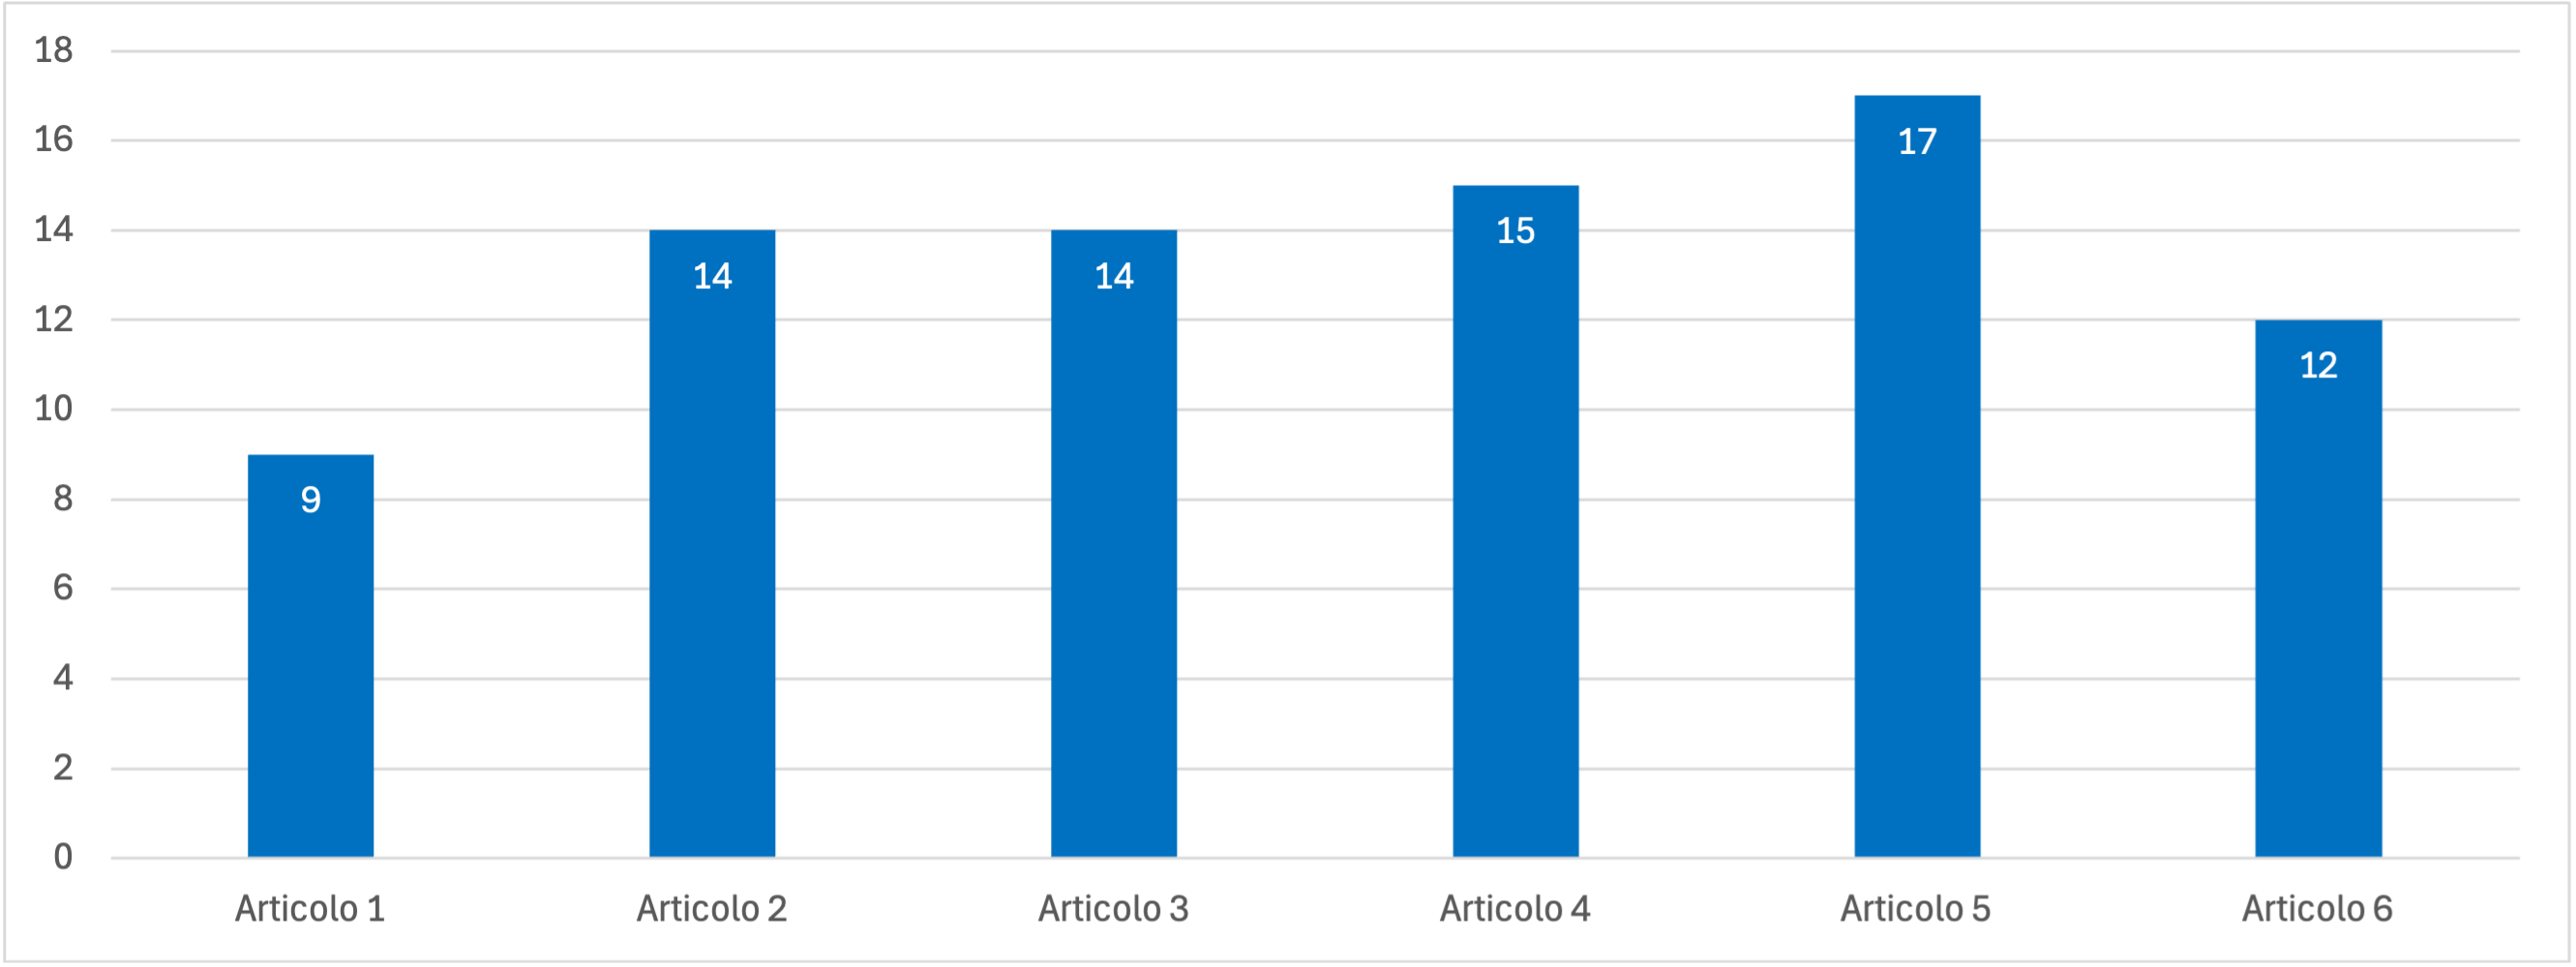
\includegraphics[width=1\linewidth]{Immagini/Istogramma Articoli.png}
    \caption{Istogramma articoli.}
    \label{fig:istogramma-articoli}
\end{figure}
    \chapter{Analisi degli eventi}
\section{Rally a Indianola, Iowa (14 gennaio 2024)}

Il 14 gennaio 2024 a Indianola, presso il Simpson College in Iowa, si è tenuto un importante rally elettorale di Donald Trump in vista dei caucus repubblicani.
Trump ha parlato ai suoi sostenitori, promettendo misure ancora più dure rispetto al passato, tra cui un forte rilancio della produzione di petrolio, deportazioni di immigrati irregolari e una politica estera improntata a rapporti diretti con leader come Putin e Kim Jong-un.
L’evento si è svolto in un clima molto freddo, ma ha visto una grande partecipazione di pubblico, sottolineando l’importanza dell’Iowa come primo stato a votare nelle primarie USA 2024.
Il rally ha avuto anche lo scopo di motivare i sostenitori a partecipare attivamente ai caucus del giorno successivo, fondamentali per la corsa alla nomination repubblicana. \\

\begin{figure}[H]
    \centering
    \begin{subfigure}[t]{0.48\textwidth}
        \centering
        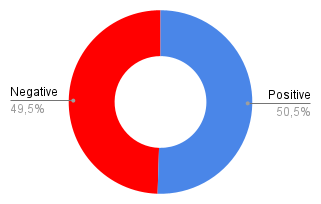
\includegraphics[width=\linewidth]{Immagini//Articolo1/Articolo 1 - Rapporto Totale Parole.png}
        \caption{Distribuzione del sentiment nelle parole analizzate.}
        \label{fig:totale-parole-a1}
    \end{subfigure}
    \hfill
    \begin{subfigure}[t]{0.48\textwidth}
        \centering
        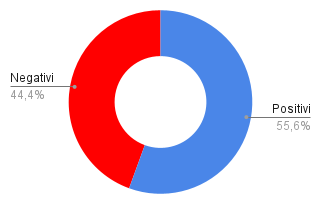
\includegraphics[width=\linewidth]{Immagini//Articolo1/Articolo 1 - Rapporto Totale Articoli.png}
        \caption{Distribuzione degli articoli per orientamento politico.}
        \label{fig:totale-articoli-a1}
    \end{subfigure}
    \caption{Articolo 1 - Analisi complessiva del corpus: parole e articoli.}
    \label{fig:analisi-totale-a1}

    \centering
    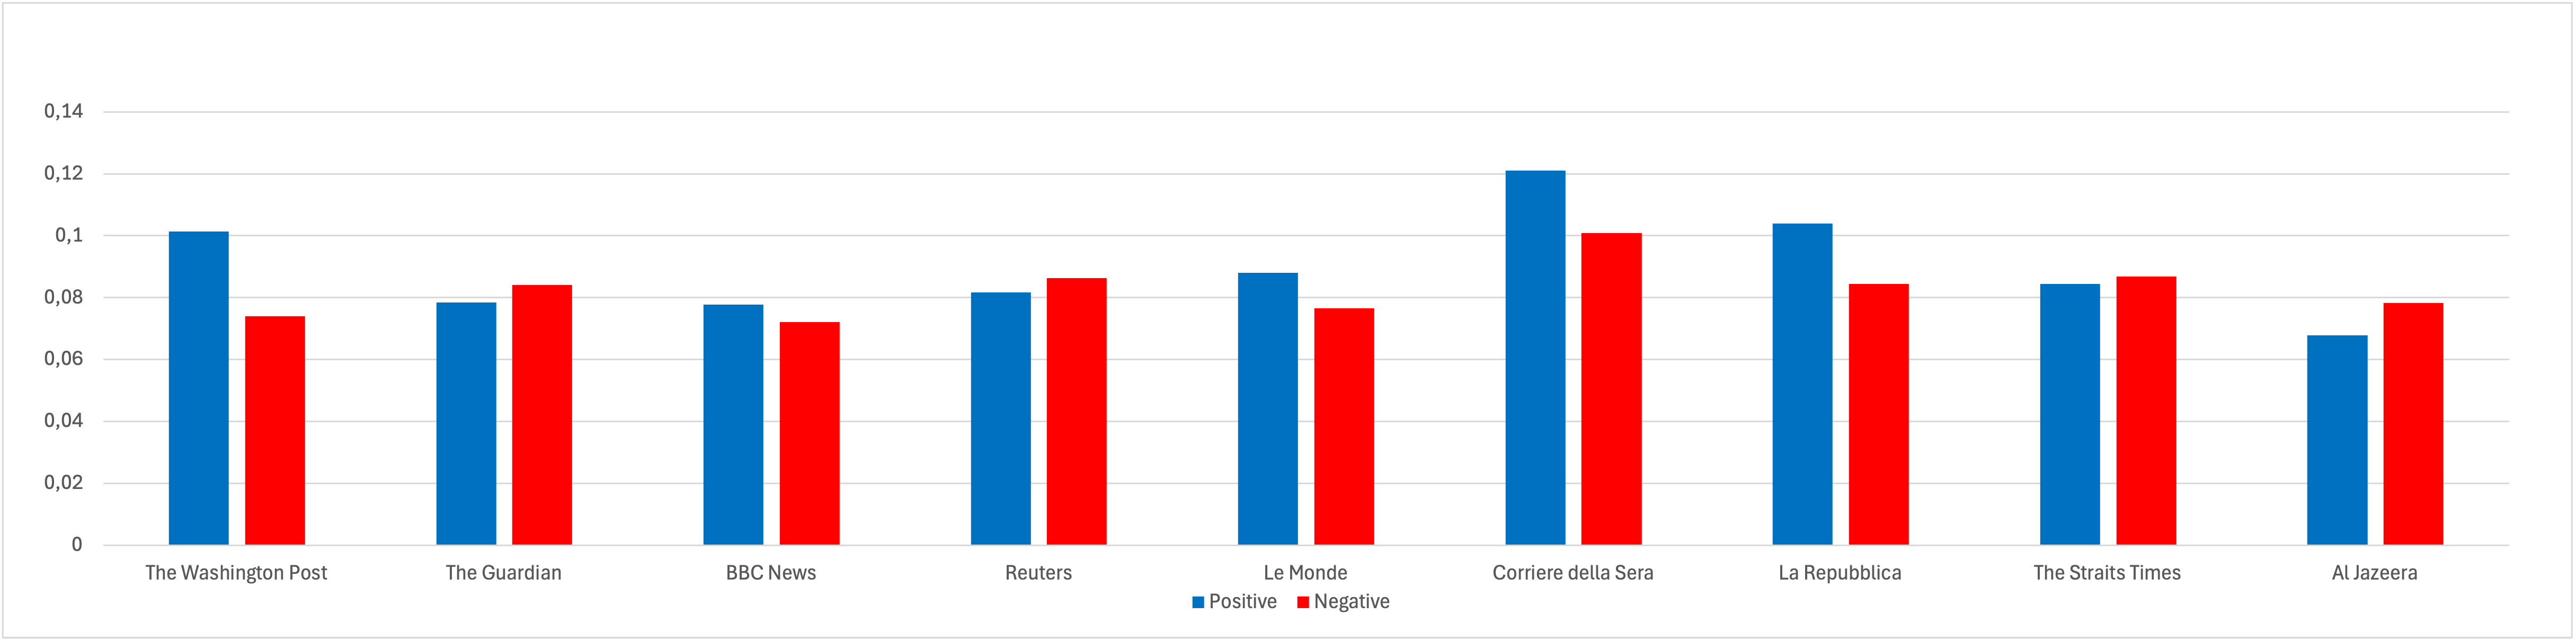
\includegraphics[width=1\linewidth]{Immagini//Articolo1/Articolo 1 - Analisi Grafica Risultati Totali.png}
    \caption{Articolo 1 - Distribuzione del sentiment negli articoli analizzati: confronto tra parole positive e negative.}
    \label{fig:risultati-totali-a1}
\end{figure}

I risultati illustrati evidenziano una distribuzione lessicale sostanzialmente bilanciata tra termini a connotazione positiva (\SI{50.5}{\percent}) e negativa (\SI{49.5}{\percent}) come evidenziato nella Figura~\ref{fig:totale-parole-a1}. Tale equilibrio linguistico suggerisce una narrazione mediatica complessivamente neutra dal punto di vista puramente semantico. Tuttavia, nonostante questa apparente neutralità, l'analisi del tono generale degli articoli (Figura~\ref{fig:totale-articoli-a1}) mostra che 5 articoli su 9, il \SI{55.6}{\percent}, assumono un'impostazione prevalentemente positiva, mentre 4 articoli su 9, il \SI{44.4}{\percent}, si caratterizza con un orientamento negativo.
Questa discrepanza tra il bilanciamento lessicale e la valutazione del tono complessivo (visualizzata graficamente nella Figura~\ref{fig:analisi-totale-a1}) può essere ricondotta a diversi fattori, tra cui il peso semantico attribuito alle parole chiave all'interno del contesto testuale, nonché la presenza di giudizi ambivalenti o contrastanti all'interno dei singoli articoli.
Per quanto riguarda l'orientamento politico delle fonti esaminate, la distribuzione risulta relativamente omogenea: si rilevano infatti quattro articoli provenienti da testate neutrali, tre da fonti con orientamento progressista e due da fonti di matrice conservatrice. Tale composizione suggerisce una copertura mediatica equilibrata, seppur con una lieve inclinazione critica.

\newpage
\section{Discorso al CPAC (24 febbraio 2024)}

Al CPAC 2024, tenutosi il 24 febbraio al National Harbor (Maryland), Donald Trump ha tenuto un discorso molto atteso davanti ai principali esponenti del movimento conservatore americano.
Nel suo intervento, Trump si è definito un “dissidente politico” e ha presentato le elezioni del 5 novembre come una sorta di “giorno della liberazione” per gli Stati Uniti.
Ha attaccato duramente l’amministrazione Biden, promesso di “salvare l’America” e ha ribadito i suoi temi chiave: lotta all’immigrazione irregolare, difesa dei valori tradizionali, revisione delle politiche economiche e dure critiche contro l’establishment di Washington.
Il discorso ha galvanizzato la platea, confermando il ruolo centrale di Trump nel partito repubblicano e tra i conservatori americani. \\

\begin{figure}[H]
    \centering
    \begin{subfigure}[t]{0.48\textwidth}
        \centering
        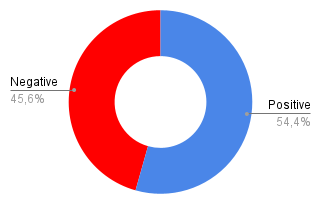
\includegraphics[width=\linewidth]{Immagini//Articolo2/Articolo 2 - Rapporto Totale Parole.png}
        \caption{Distribuzione del sentiment nelle parole analizzate.}
        \label{fig:totale-parole-a2}
    \end{subfigure}
    \hfill
    \begin{subfigure}[t]{0.48\textwidth}
        \centering
        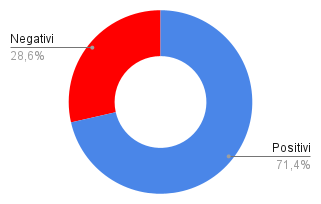
\includegraphics[width=\linewidth]{Immagini//Articolo2/Articolo 2 - Rapporto Totale Articoli.png}
        \caption{Distribuzione degli articoli per orientamento politico.}
        \label{fig:totale-articoli-a2}
    \end{subfigure}
    \caption{Articolo 2 - Analisi complessiva del corpus: parole e articoli.}
    \label{fig:analisi-totale-a2}

    \centering
    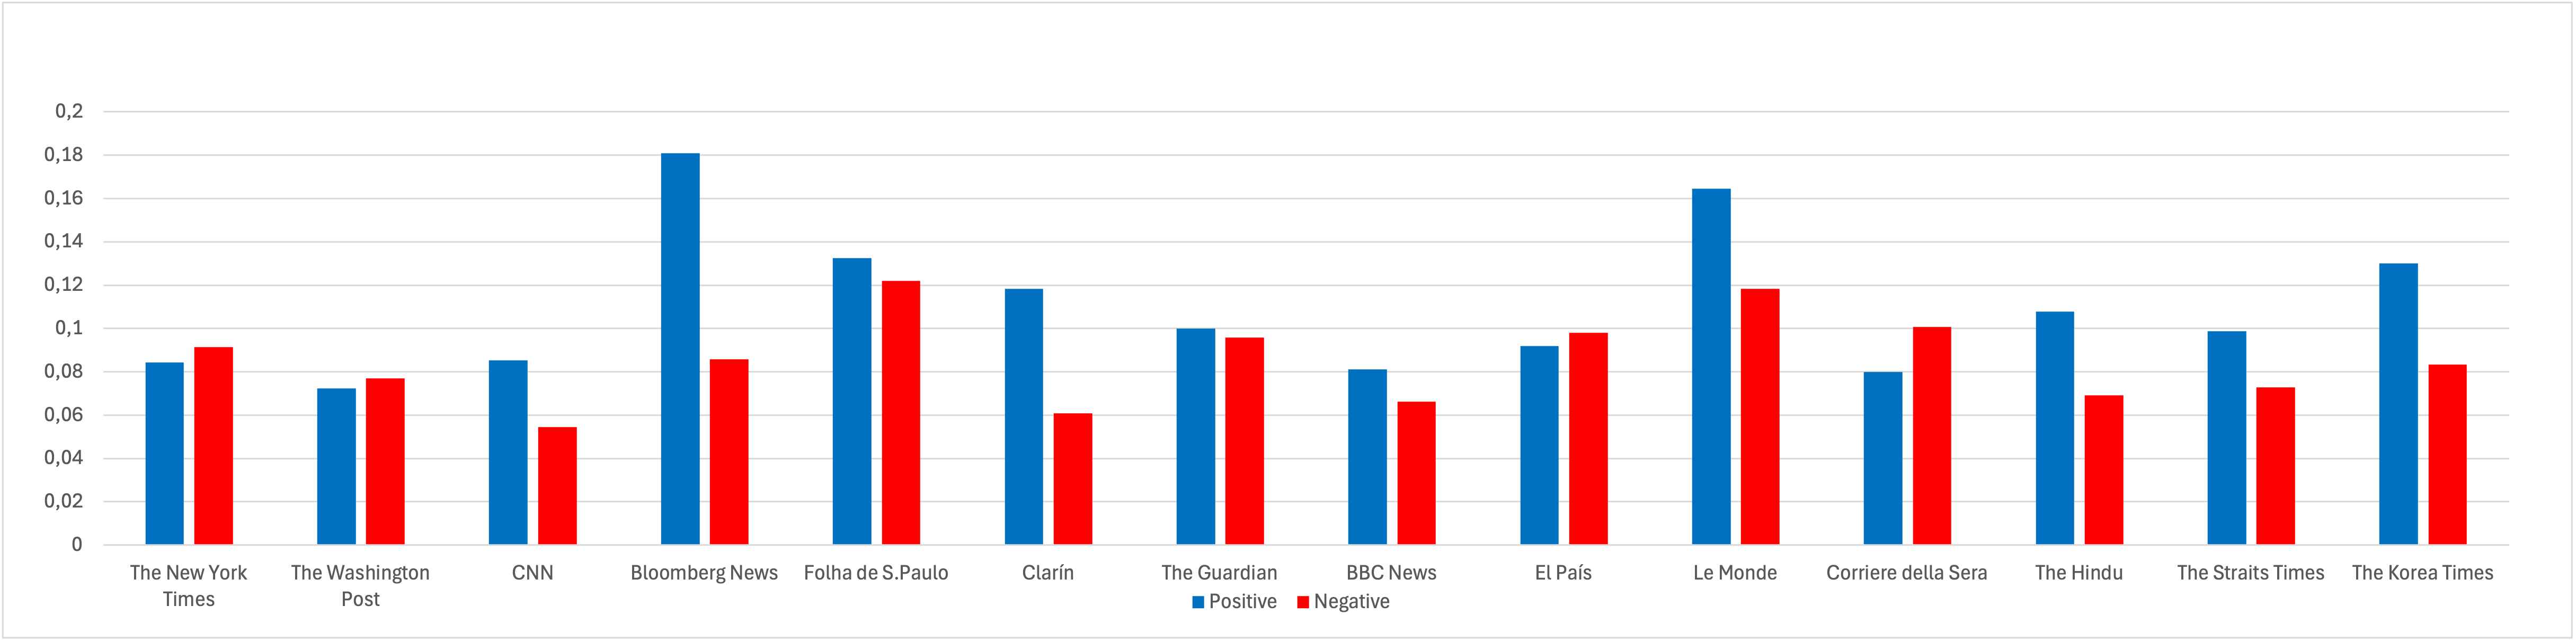
\includegraphics[width=1\linewidth]{Immagini//Articolo2/Articolo 2 - Analisi Grafica Risultati Totali.png}
    \caption{Articolo 2 - Distribuzione del sentiment negli articoli analizzati: confronto tra parole positive e negative.}
    \label{fig:risultati-totali-a2}
\end{figure}

In questo caso vi è una prevalenza di articoli provenienti da testate progressiste (6), rispetto a quelli riconducibili a fonti conservatrici (5) e neutrali (3). Tale distribuzione suggerisce una copertura mediatica leggermente orientata verso una prospettiva progressista, che potrebbe influenzare il tono complessivo della narrazione.
L'analisi del sentiment lessicale (Figura~\ref{fig:totale-parole-a2}) mostra una predominanza di termini a connotazione positiva (\SI{54.4}{\percent}) rispetto a quelli negativi (\SI{45.6}{\percent}), questo si riflette anche nel tono generale degli articoli (Figura~\ref{fig:totale-articoli-a2}), dove la maggioranza (10 articoli su 14, pari al \SI{71.4}{\percent}) è stata classificata come positiva, mentre solo 4 articoli (\SI{28.6}{\percent}) risultano avere un tono negativo.
Dal punto di vista delle parole utilizzate, il rapporto tra termini positivi e negativi suggerisce una narrazione favorevole, in linea con la classificazione degli articoli. Da notare che anche testate generalmente considerate neutrali o conservatrici hanno espresso, in vari casi, un tono positivo.
In conclusione, la copertura mediatica del discorso al CPAC 2024 appare complessivamente positiva, sia in termini quantitativi (numero di articoli con tono favorevole) sia qualitativi (prevalenza di lessico positivo), nonostante la leggera prevalenza di fonti progressiste. Ciò suggerisce una ricezione generalmente benevola del contenuto del discorso, indipendentemente dall’orientamento politico delle testate analizzate.

\newpage
\section{Nomination repubblicana (18 luglio 2024)}
Il 18 luglio 2024, a Milwaukee, Donald Trump ha accettato la nomination repubblicana alla presidenza, pochi giorni dopo un attentato in cui è rimasto ferito. Con una benda sull'orecchio, ha promesso di "salvare l'America", unire il paese e ripristinare il "sogno americano". 
Pur aprendo con toni più concilianti, ha poi attaccato i democratici e ribadito le sue promesse classiche: chiusura delle frontiere, deportazioni, rilancio del petrolio e tagli alle tasse.
Il discorso si è concluso in un clima di entusiasmo con una pioggia di palloncini. \\

\begin{figure}[H]
    \centering
    \begin{subfigure}[t]{0.48\textwidth}
        \centering
        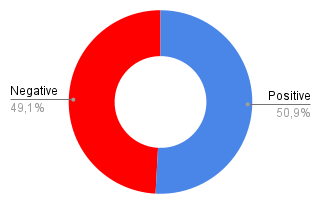
\includegraphics[width=\linewidth]{Immagini//Articolo3/Articolo 3 - Rapporto Totale Parole.png}
        \caption{Distribuzione del sentiment nelle parole analizzate.}
        \label{fig:totale-parole-a3}
    \end{subfigure}
    \hfill
    \begin{subfigure}[t]{0.48\textwidth}
        \centering
        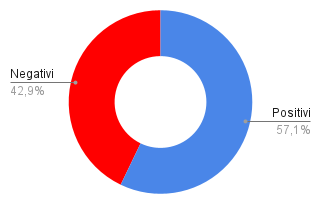
\includegraphics[width=\linewidth]{Immagini//Articolo3/Articolo 3 - Rapporto Totale Articoli.png}
        \caption{Distribuzione degli articoli per orientamento politico.}
        \label{fig:totale-articoli-a3}
    \end{subfigure}
    \caption{Articolo 3 - Analisi complessiva del corpus: parole e articoli.}
    \label{fig:analisi-totale-a3}

    \centering
    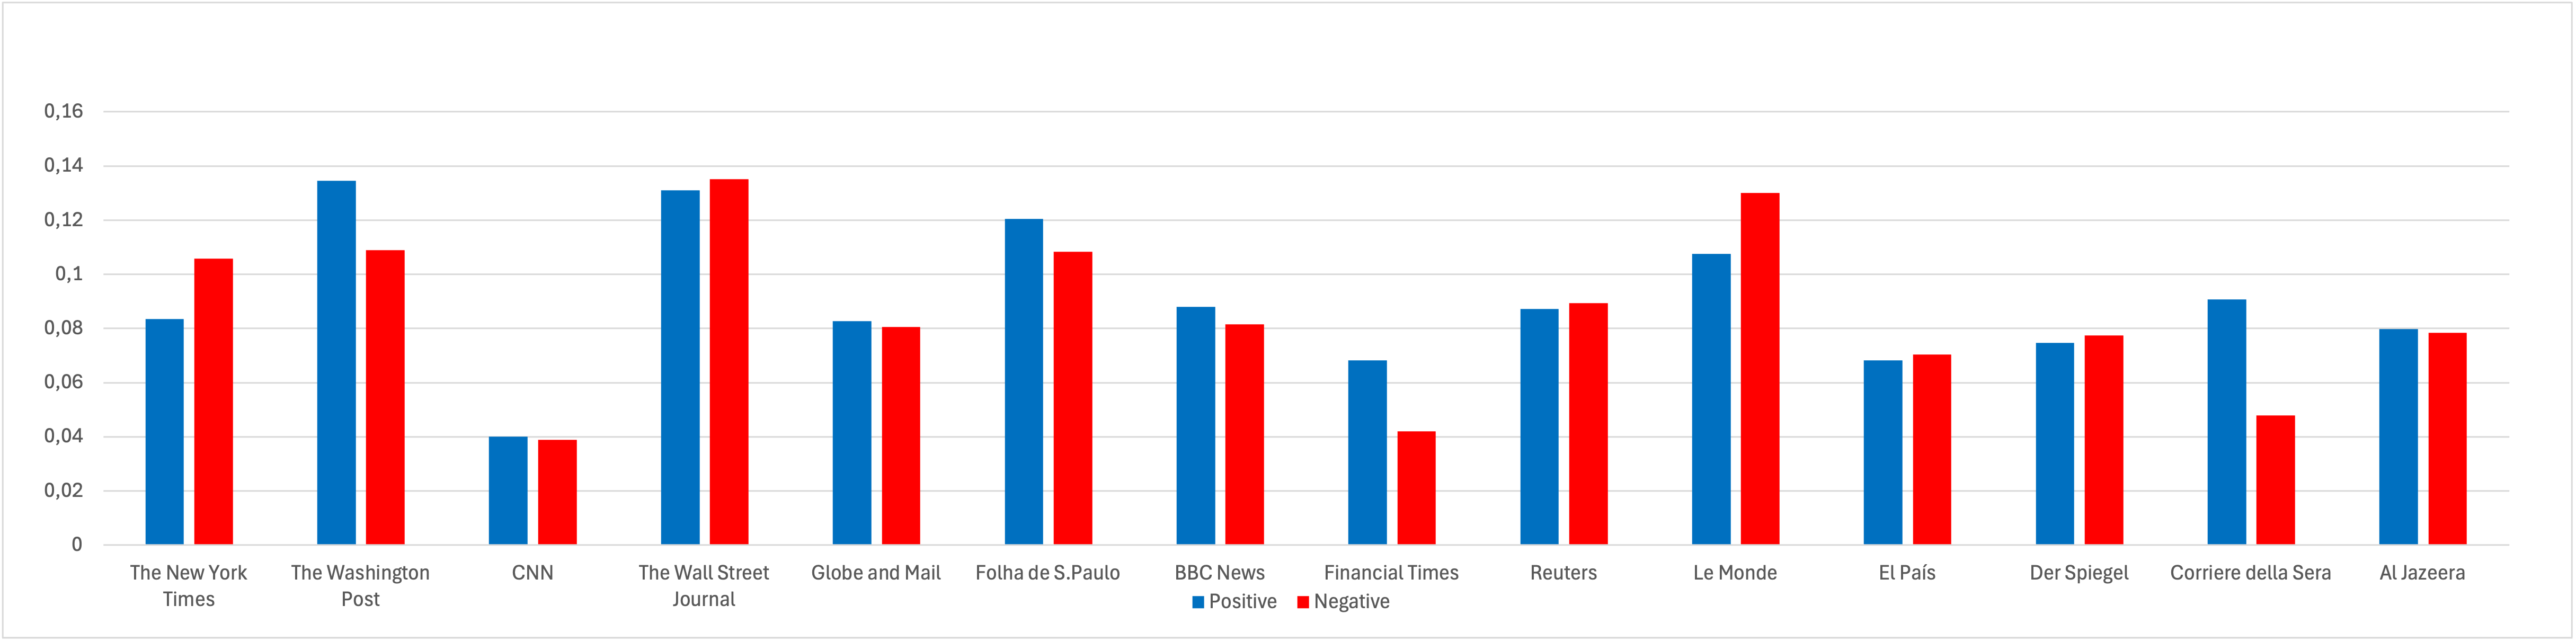
\includegraphics[width=1\linewidth]{Immagini//Articolo3/Articolo 3 - Analisi Grafica Risultati Totali.png}
    \caption{Articolo 3 - Distribuzione del sentiment negli articoli analizzati: confronto tra parole positive e negative.}
    \label{fig:risultati-totali-a3}
\end{figure}
In questo caso vi è una netta predominanza di articoli progressisti (8) rispetto a quelli neutrali (4) e conservatori (2), indicando una copertura mediatica fortemente polarizzata. Nonostante questa asimmetria politica, l'analisi lessicale (Figura~\ref{fig:totale-parole-a3}) rivela un sostanziale equilibrio tra termini positivi (\SI{50.9}{\percent}) e negativi (\SI{49.1}{\percent}), suggerendo che il linguaggio utilizzato mantiene un'apparente neutralità semantica. Tuttavia, il tono complessivo degli articoli (Figura~\ref{fig:totale-articoli-a3}) presenta una lieve differenza: 8 articoli su 14, il \SI{57.1}{\percent}, sono stati classificati come positivi contro i 6 su 14, \SI{42.9}{\percent}, negativi. Questa divergenza potrebbe derivare dall'enfasi posta dai media progressisti sugli aspetti drammatici dell'attentato subito da Trump (citato come elemento negativo in contesti positivi) o dalla tendenza dei conservatori a celebrare il "miracoloso salvataggio" come simbolo di resilienza, dimostrando come eventi traumatici possano generare narrazioni complesse dove elementi critici e positivi si intrecciano in modo controintuitivo.

\newpage
\section{Discorso di vittoria (6 novembre 2024)}

La notte del 6 novembre 2024, a West Palm Beach, Donald Trump ha tenuto il suo discorso di vittoria dopo le elezioni presidenziali.
Ha parlato di “età dell’oro per l’America”, promettendo di mantenere le sue promesse, unire il Paese e “fermare le guerre”.
Ha ringraziato la famiglia, i sostenitori e ha definito la sua vittoria “il più grande comeback della storia”, sottolineando il mandato ricevuto dagli americani e la conquista di diversi stati chiave.
Ha elogiato Elon Musk e ha promesso che l’America tornerà grande. \\

\begin{figure}[H]
    \centering
    \begin{subfigure}[t]{0.48\textwidth}
        \centering
        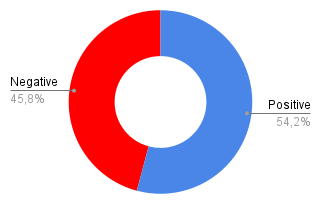
\includegraphics[width=\linewidth]{Immagini//Articolo4/Articolo 4 - Rapporto Totale Parole.png}
        \caption{Distribuzione del sentiment nelle parole analizzate.}
        \label{fig:totale-parole-a4}
    \end{subfigure}
    \hfill
    \begin{subfigure}[t]{0.48\textwidth}
        \centering
        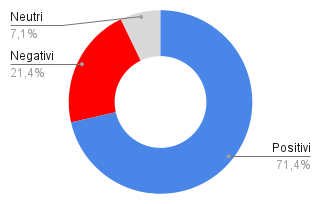
\includegraphics[width=\linewidth]{Immagini//Articolo4/Articolo 4 - Rapporto Totale Articoli.png}
        \caption{Distribuzione degli articoli per orientamento politico.}
        \label{fig:totale-articoli-a4}
    \end{subfigure}
    \caption{Articolo 4 - Analisi complessiva del corpus: parole e articoli.}
    \label{fig:analisi-totale-a4}

    \centering
    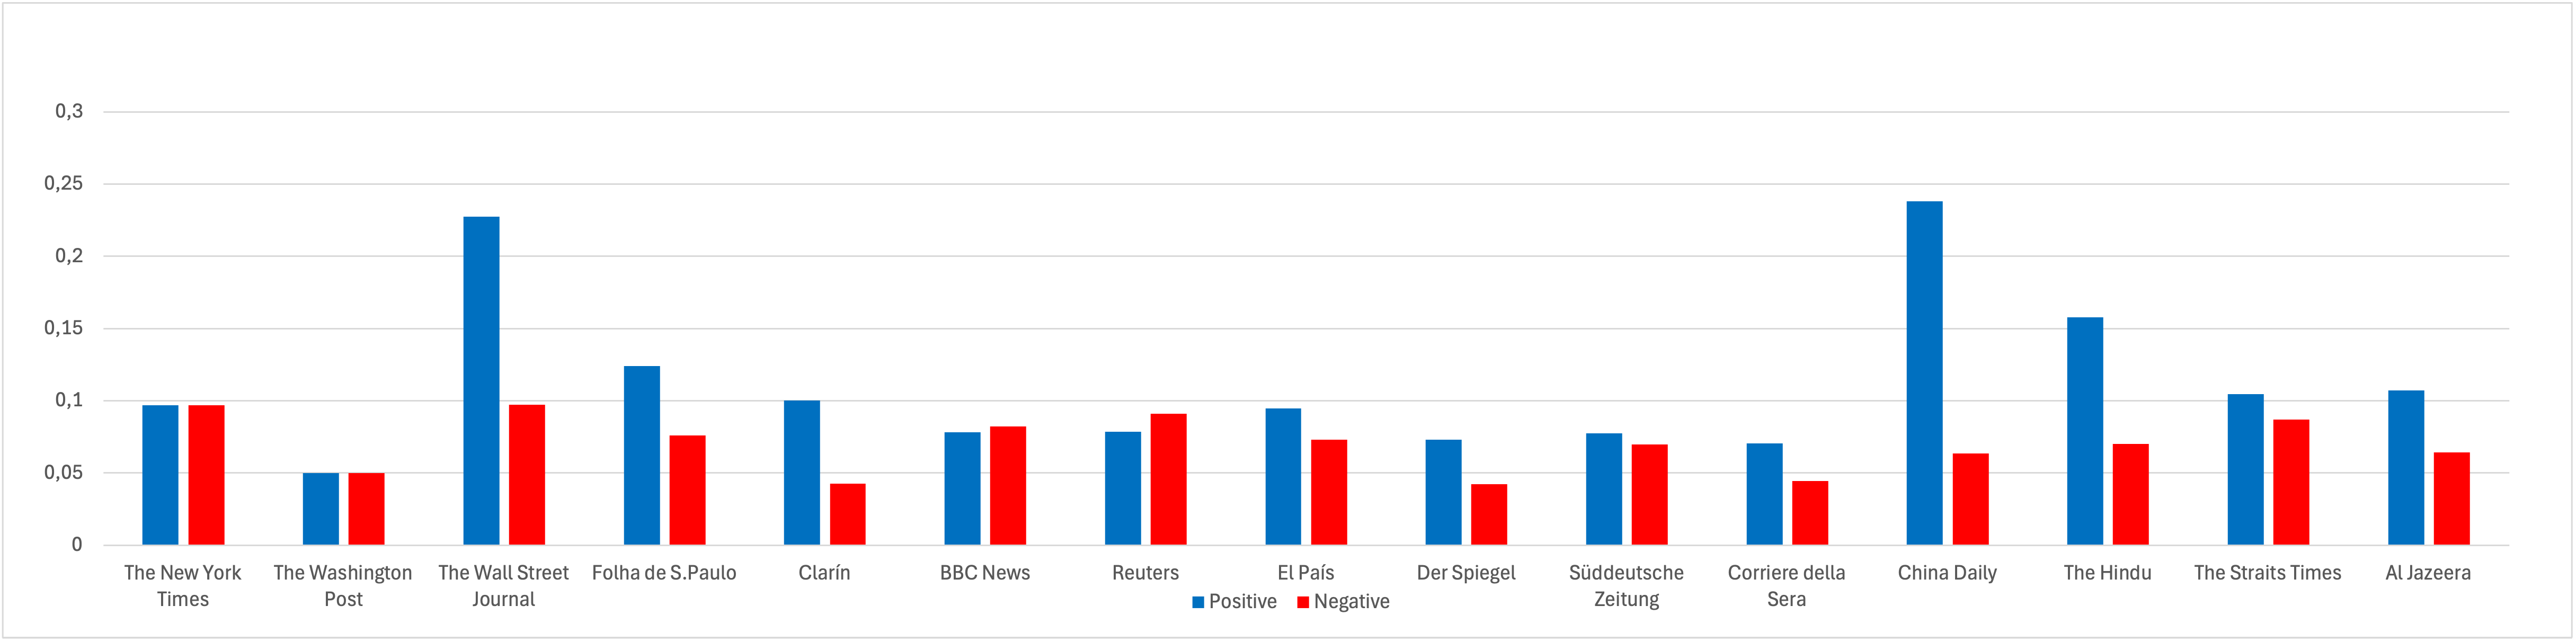
\includegraphics[width=1\linewidth]{Immagini//Articolo4/Articolo 4 - Analisi Grafica Risultati Totali.png}
    \caption{Articolo 4 - Distribuzione del sentiment negli articoli analizzati: confronto tra parole positive e negative.}
    \label{fig:risultati-totali-a4}
\end{figure}
L'analisi del discorso di vittoria elettorale rivela una marcata polarizzazione nel tono degli articoli, con una schiacciante maggioranza di contenuti positivi, 10 articoli su 14 (\SI{71.8}{\percent}), rispetto a quelli negativi, 3 articoli su 14 (\SI{21.4}{\percent}), e neutrali, 1 articolo su 14 (\SI{7}{\percent}) (Figura~\ref{fig:totale-articoli-a4}). Questo quadro contrasta parzialmente con l'analisi lessicale (Figura~\ref{fig:totale-parole-a4}), che mostra un equilibrio più moderato tra termini positivi (\SI{54.2}{\percent}) e negativi (\SI{45.8}{\percent}). La discrepanza evidenzia come elementi contestuali - come il clima di celebrazione post-elettorale e le immagini simboliche della vittoria - abbiano influenzato il tono complessivo oltre la mera frequenza di parole polarizzate. Particolarmente significativo è il minimo apporto di articoli neutrali (1 articolo su 14, il \SI{7}{\percent}), che suggerisce come l'evento abbia spinto i media a prendere posizione netta, sia in senso celebrativo (specialmente tra i conservatori) sia critico (tra i progressisti). L'uso strategico di espressioni come "età dell'oro" da parte di Trump par aver funzionato come frame dominante, mentre le critiche sono state relegate a un ruolo minoritario nonostante costituissero quasi la metà del lessico utilizzato.

\newpage
\section{Discorso inaugurale (20 gennaio 2025)}

Il 20 gennaio 2025, Donald Trump ha tenuto il discorso di insediamento come 47º Presidente degli Stati Uniti a Washington.
Ha dichiarato che “l’Età dell’Oro dell’America inizia proprio ora”, promettendo di mettere “America al primo posto”, ripristinare la sovranità, la sicurezza e la giustizia, e porre fine all’uso politico del Dipartimento di Giustizia.
Ha annunciato una “rivoluzione del buon senso”, la dichiarazione di emergenza nazionale al confine sud, il ritorno della politica “Remain in Mexico”, la lotta ai cartelli della droga e il rilancio della produzione energetica nazionale.
Ha ringraziato le comunità nere e ispaniche per il sostegno, ha promesso unità nazionale e ha sottolineato che “il declino dell’America è finito”.
Ha concluso affermando che il suo obiettivo sarà essere “pacificatore e unificatore”, rilanciando il sogno americano e la fiducia nel futuro del Paese.

\begin{figure}[H]
    \centering
    \begin{subfigure}[t]{0.48\textwidth}
        \centering
        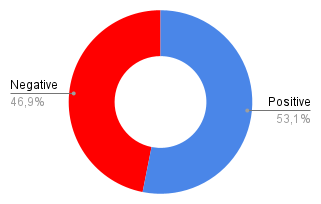
\includegraphics[width=\linewidth]{Immagini//Articolo5/Articolo 5 - Rapporto Totale Parole.png}
        \caption{Distribuzione del sentiment nelle parole analizzate.}
        \label{fig:totale-parole-a5}
    \end{subfigure}
    \hfill
    \begin{subfigure}[t]{0.48\textwidth}
        \centering
        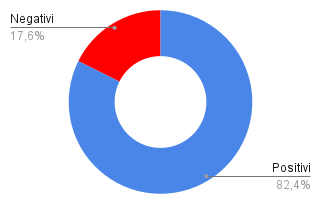
\includegraphics[width=\linewidth]{Immagini//Articolo5/Articolo 5 - Rapporto Totale Articoli.png}
        \caption{Distribuzione degli articoli per orientamento politico.}
        \label{fig:totale-articoli-a5}
    \end{subfigure}
    \caption{Articolo 5 - Analisi complessiva del corpus: parole e articoli.}
    \label{fig:analisi-totale-a5}

    \centering
    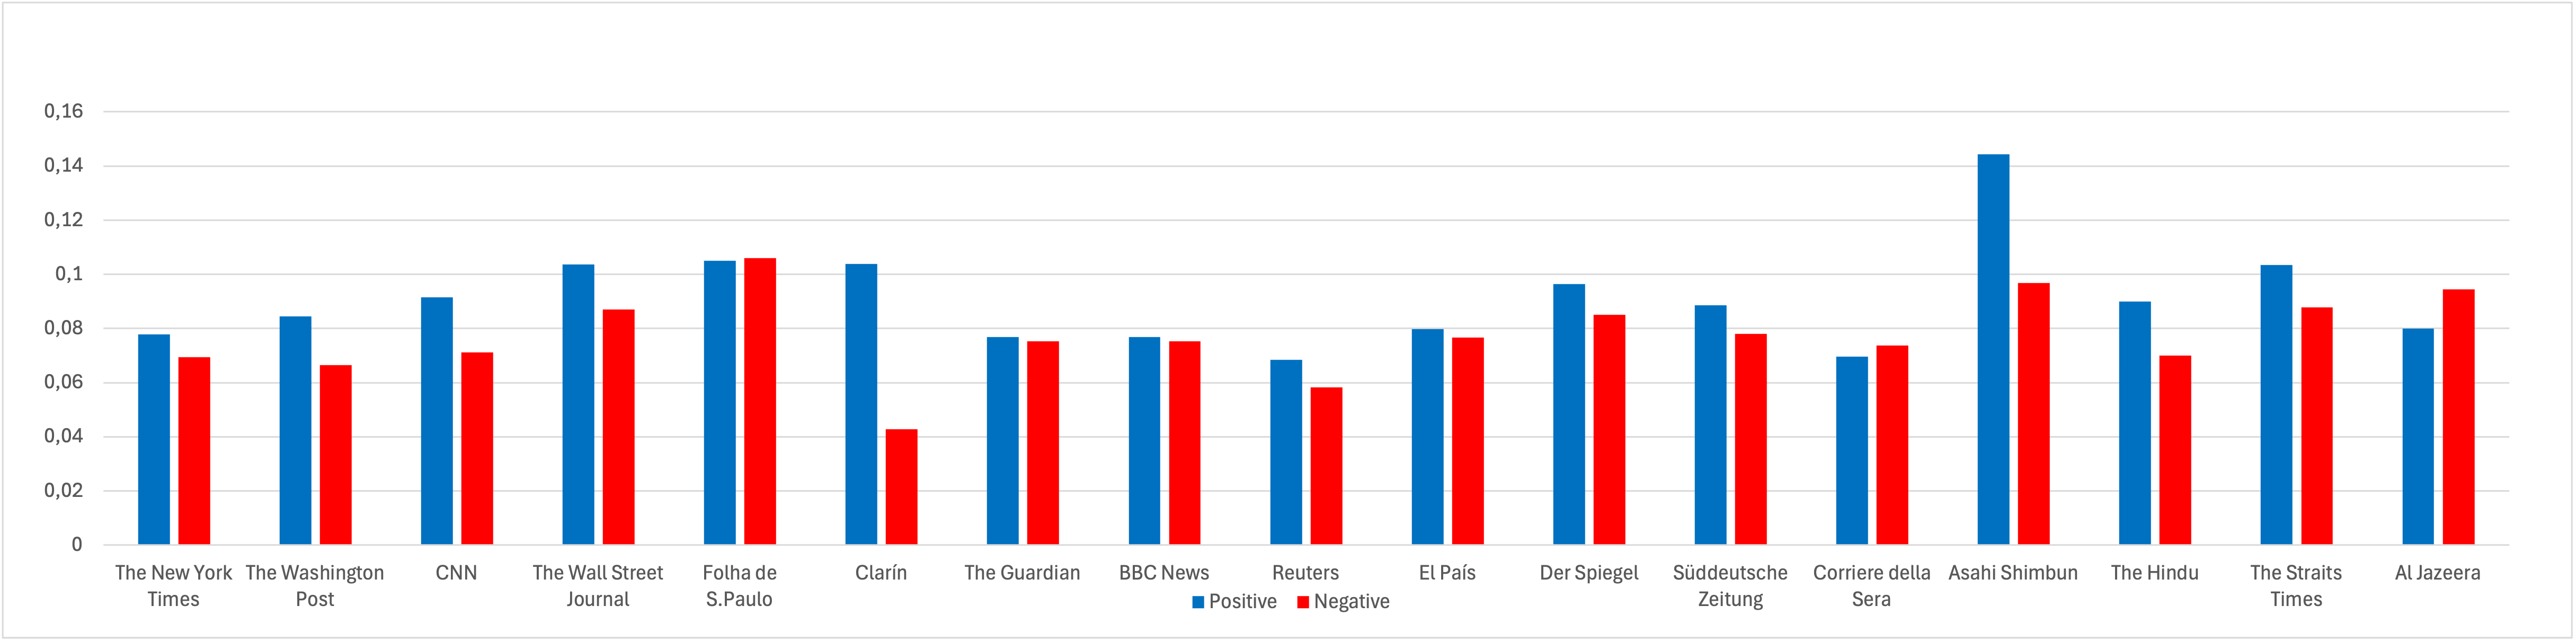
\includegraphics[width=1\linewidth]{Immagini//Articolo5/Articolo 5 - Analisi Grafica Risultati Totali.png}
    \caption{Articolo 5 - Distribuzione del sentiment negli articoli analizzati: confronto tra parole positive e negative.}
    \label{fig:risultati-totali-a5}
\end{figure}
L'analisi del discorso inaugurale mostra una predominanza di articoli progressisti (8 su 17) rispetto a quelli neutrali (5 su 17) e conservatori (4 su 17), indicando una copertura mediatica con significativa polarizzazione politica. Nonostante tale squilibrio, l'analisi lessicale (Figura~\ref{fig:totale-parole-a5}) rivela un lieve vantaggio dei termini positivi (\SI{53.1}{\percent}) rispetto a quelli negativi (\SI{46.9}{\percent}), riflettendo probabilmente il tono istituzionale ed unificante tipico di un discorso d'insediamento. Sorprendentemente, il \SI{82.4}{\percent} degli articoli è stato classificato come positivo nel tono complessivo, contro solo il \SI{17.6}{\percent} negativo (Figura~\ref{fig:totale-articoli-a6}). Questa marcata discrepanza tra la significativa presenza di lessico negativo e il tono prevalentemente positivo degli articoli può essere spiegata attraverso tre fattori chiave: 
\begin{enumerate}
    \item L'uso da parte dei media progressisti di citazioni dirette del discorso (positive) in contesti critici
    \item L'enfasi mediatica sugli aspetti rituali e simbolici della cerimonia presidenziale
    \item La tendenza dei conservatori a celebrare l'evento come ripristino della tradizione
\end{enumerate}
L'estrema rarità di articoli negativi (\SI{17.6}{\percent}) suggerisce che persino i media dell'opposizione abbiano riservato un trattamento rispettoso al momento istituzionale, pur mantenendo riserve sulle politiche annunciate.

\newpage
\section{Forum economico mondiale a Davos (23 gennaio 2025)}

A Davos, il 23 gennaio 2025, Trump ha promesso una "nuova età dell'oro" per gli USA, con l'obiettivo di renderli "più forti, ricchi e uniti".
Ha criticato le politiche economiche precedenti, promettendo tagli alle tasse, meno regolamentazioni e rilancio energetico.
Ha annunciato la fine del Green New Deal e dazi per chi produce all'estero.
Ha chiesto più spesa militare alla NATO, ha rivendicato meritocrazia e libertà di parola, e ha promesso di fermare l'immigrazione illegale.
Ha sottolineato investimenti record in America e auspicato la fine della guerra in Ucraina e un ruolo USA nei negoziati di pace in Medio Oriente. \\

\begin{figure}[H]
    \centering
    \begin{subfigure}[t]{0.48\textwidth}
        \centering
        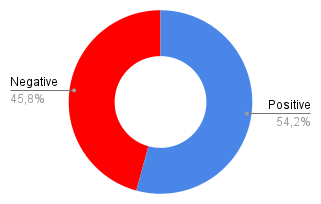
\includegraphics[width=\linewidth]{Immagini//Articolo6/Articolo 6 - Rapporto Totale Parole.png}
        \caption{Distribuzione del sentiment nelle parole analizzate.}
        \label{fig:totale-parole-a6}
    \end{subfigure}
    \hfill
    \begin{subfigure}[t]{0.48\textwidth}
        \centering
        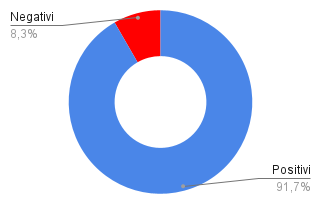
\includegraphics[width=\linewidth]{Immagini//Articolo6/Articolo 6 - Rapporto Totale Articoli.png}
        \caption{Distribuzione degli articoli per orientamento politico.}
        \label{fig:totale-articoli-a6}
    \end{subfigure}
    \caption{Articolo 6 - Analisi complessiva del corpus: parole e articoli.}
    \label{fig:analisi-totale-a6}

    \centering
    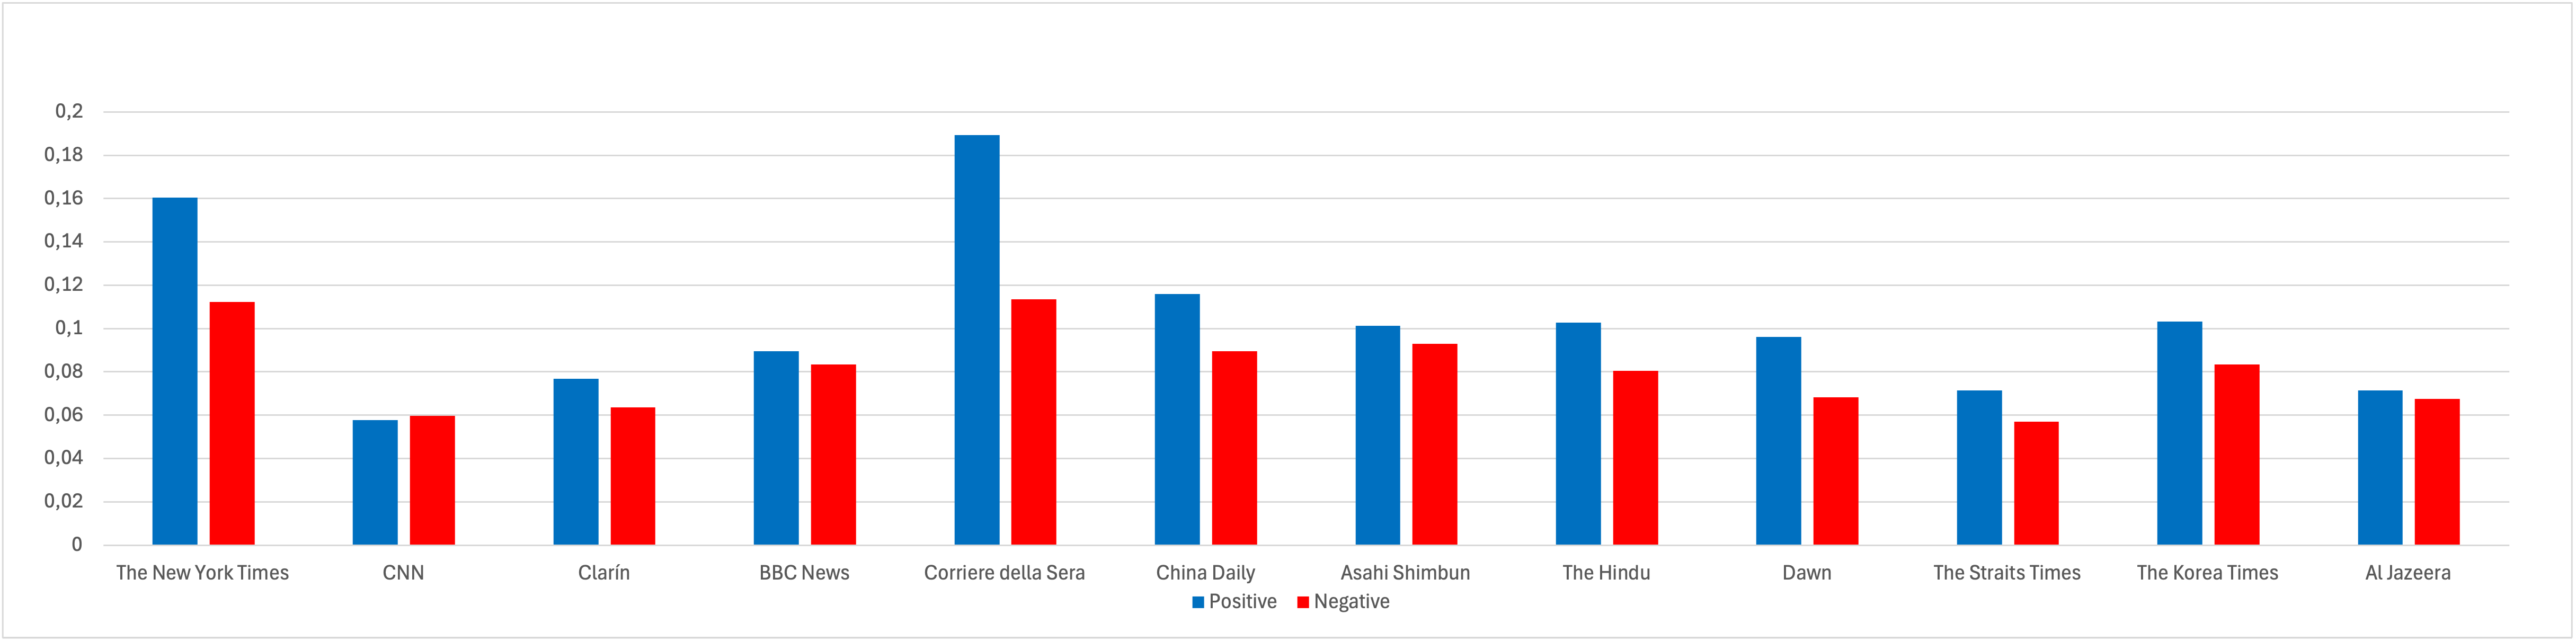
\includegraphics[width=1\linewidth]{Immagini//Articolo6/Articolo 6 - Analisi Grafica Risultati Totali.png}
    \caption{Articolo 6 - Distribuzione del sentiment negli articoli analizzati: confronto tra parole positive e negative.}
    \label{fig:risultati-totali-a6}
\end{figure}
L'analisi del discorso al World Economic Forum effettuata su una distribuzione equilibrata tra articoli progressisti, neutrali e conservatori (4 ciascuno), mostra un tono complessivo straordinariamente positivo: 11 articoli su 12, il \SI{91.7}{\percent}, sono stati classificati come favorevoli, contro solo 1 articolo su 12, l'\SI{8.3}{\percent}, critico  (Figura~\ref{fig:totale-articoli-a6}). Questo risultato contrasta parzialmente con l'analisi lessicale (Figura~\ref{fig:totale-parole-a6}), dove le parole positive (\SI{54.2}{\percent}) superano quelle negative (\SI{45.8}{\percent}) con un margine più contenuto. La marcata discrepanza tra il \SI{45.9}{\percent} di lessico negativo ed il singolo articolo critico suggerisce che: 
\begin{enumerate}
    \item I media abbiano generalmente "normalizzato" le controversie (dazi, abbandono del Green New Deal) inserendole in un frame complessivo di sviluppo economico
    \item Il contesto internazionale del WEF abbia indotto un trattamento più istituzionale
    \item La retorica trumpiana di "nuova età dell'oro" abbia funzionato da potente cornice interpretativa. 
\end{enumerate}
È particolarmente significativo come anche i media progressisti abbiano adottato prevalentemente un tono positivo, concentrando le critiche in specifici punti piuttosto che nell'interpretazione globale dell'evento.
    \chapter{Caso studio: Trump ad Alcatraz}

\section{Narrazione opposta: due articoli AI-generated}

\section{Analisi retorica comparata}
    \chapter{Risultati complessivi}

\section{Distribuzione articoli per orientamento}

\subsection{Progressisti}

\begin{figure}[H]
    \centering
    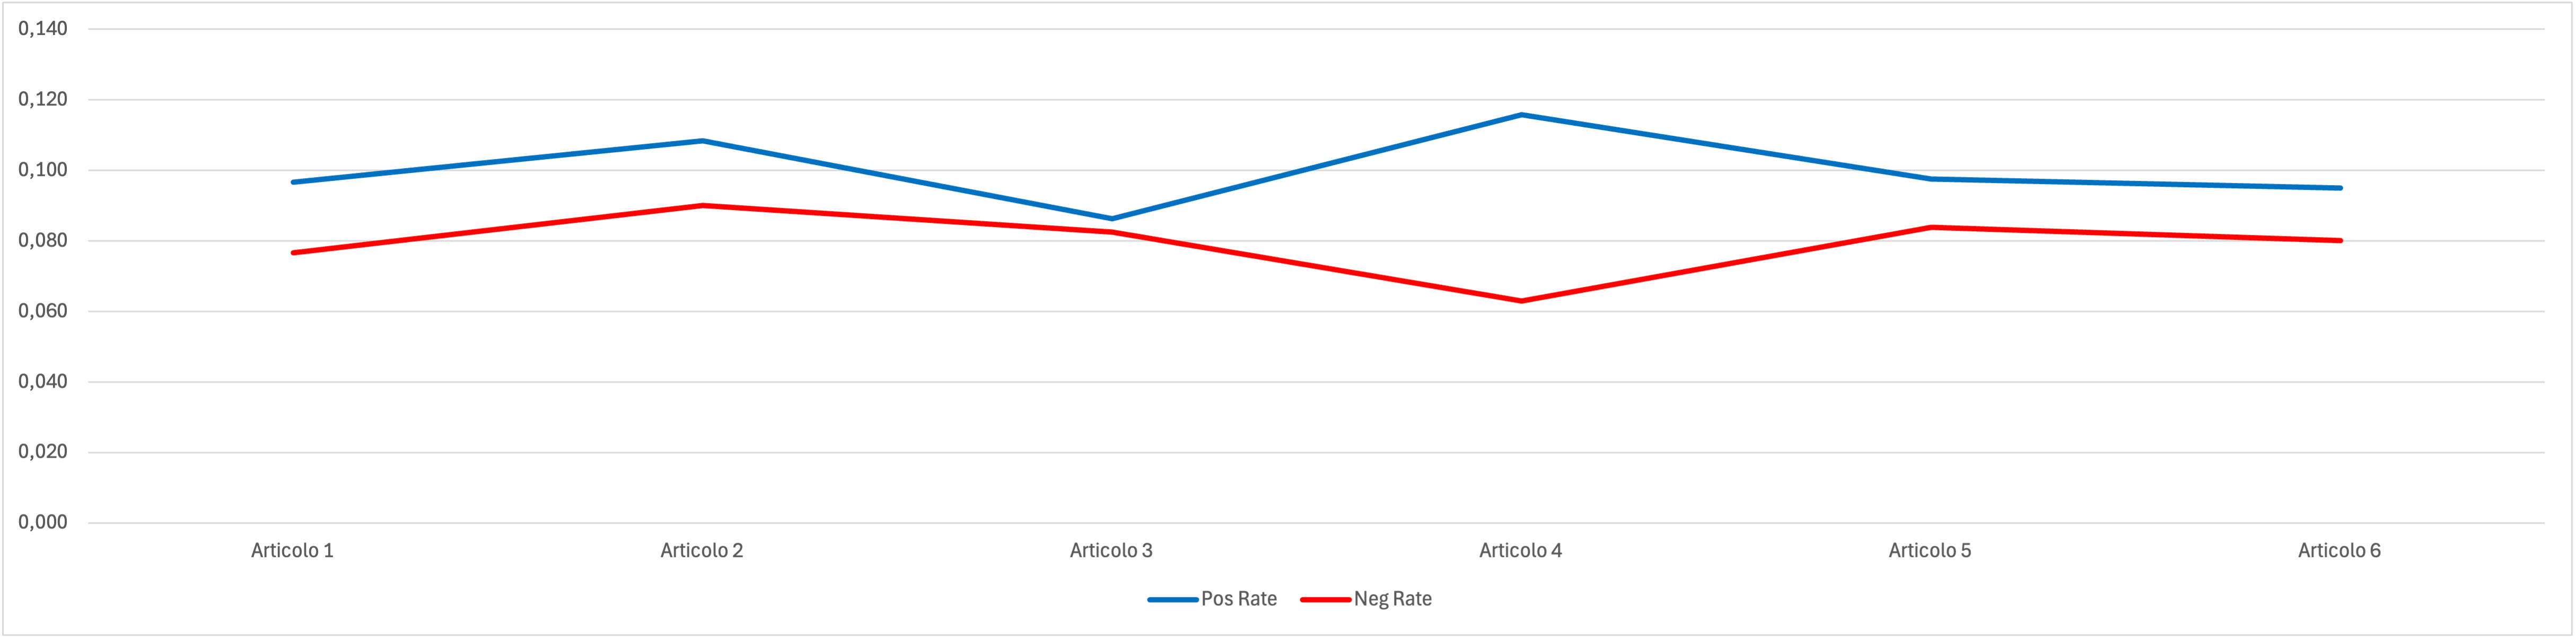
\includegraphics[width=1\linewidth]{Immagini/Progressisti/Progressisti - Sentiment Cronologico.png}
    \caption{Progressisti - Sentiment Cronologico.}
    \label{fig:enter-label-a5}

    \centering
    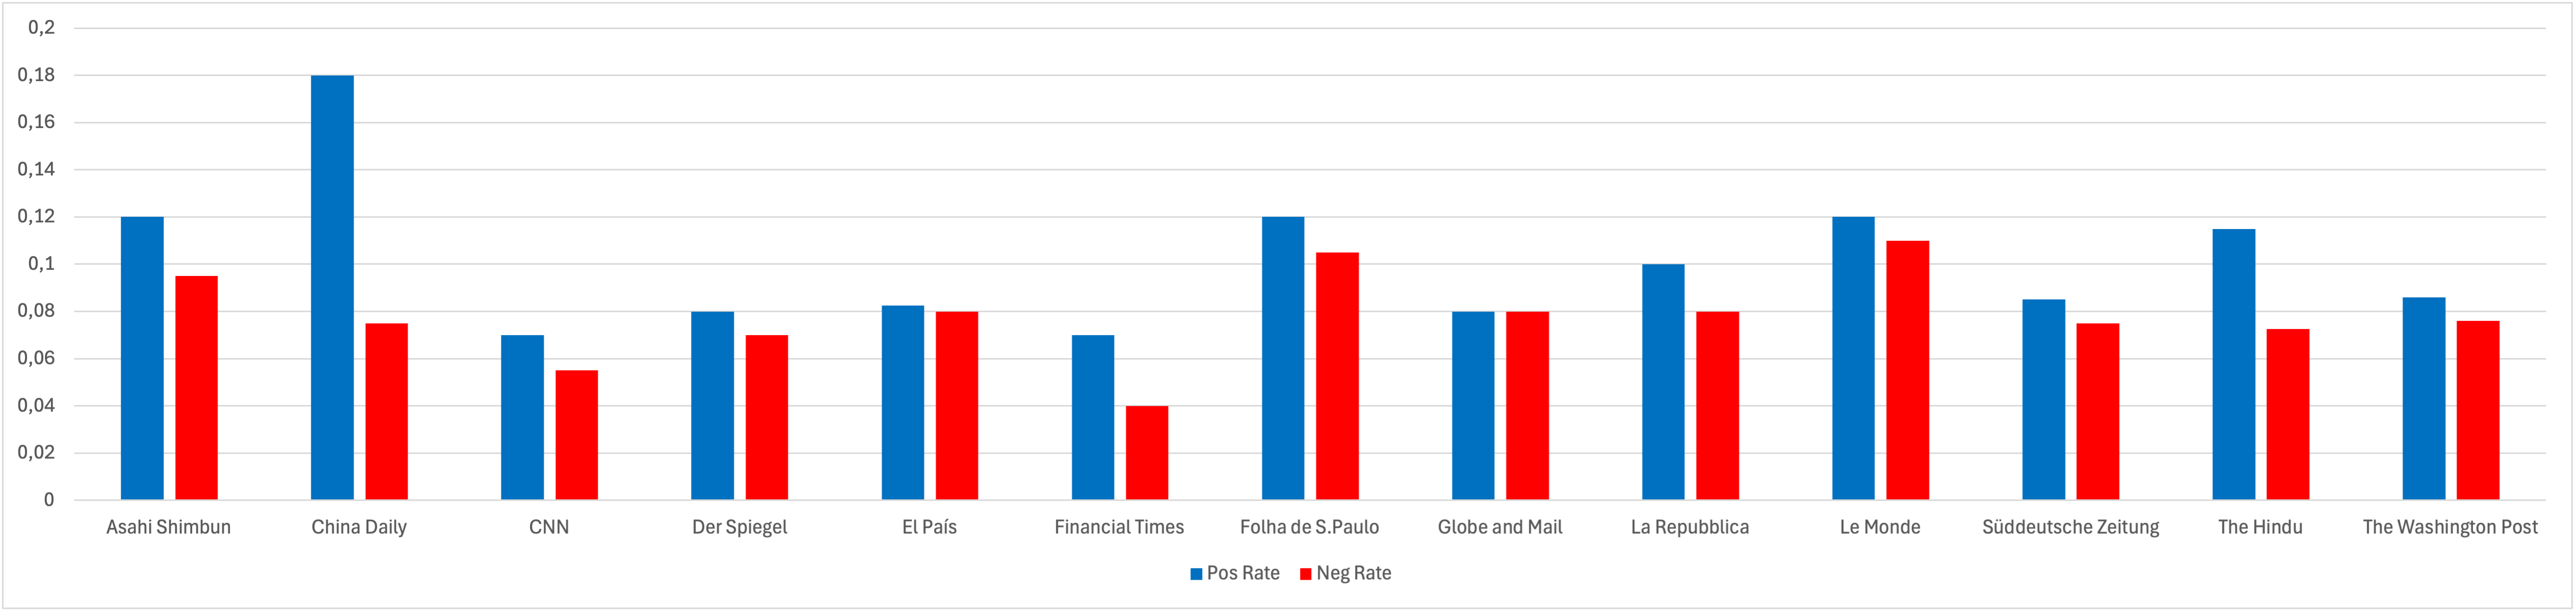
\includegraphics[width=1\linewidth]{Immagini/Progressisti/Progressisti - Sentiment Testate.png}
    \caption{Progressisti - Sentiment Testate.}
    \label{fig:enter-label-a5}
\end{figure}

\newpage
\subsection{Neutrali}

\begin{figure}[H]
    \centering
    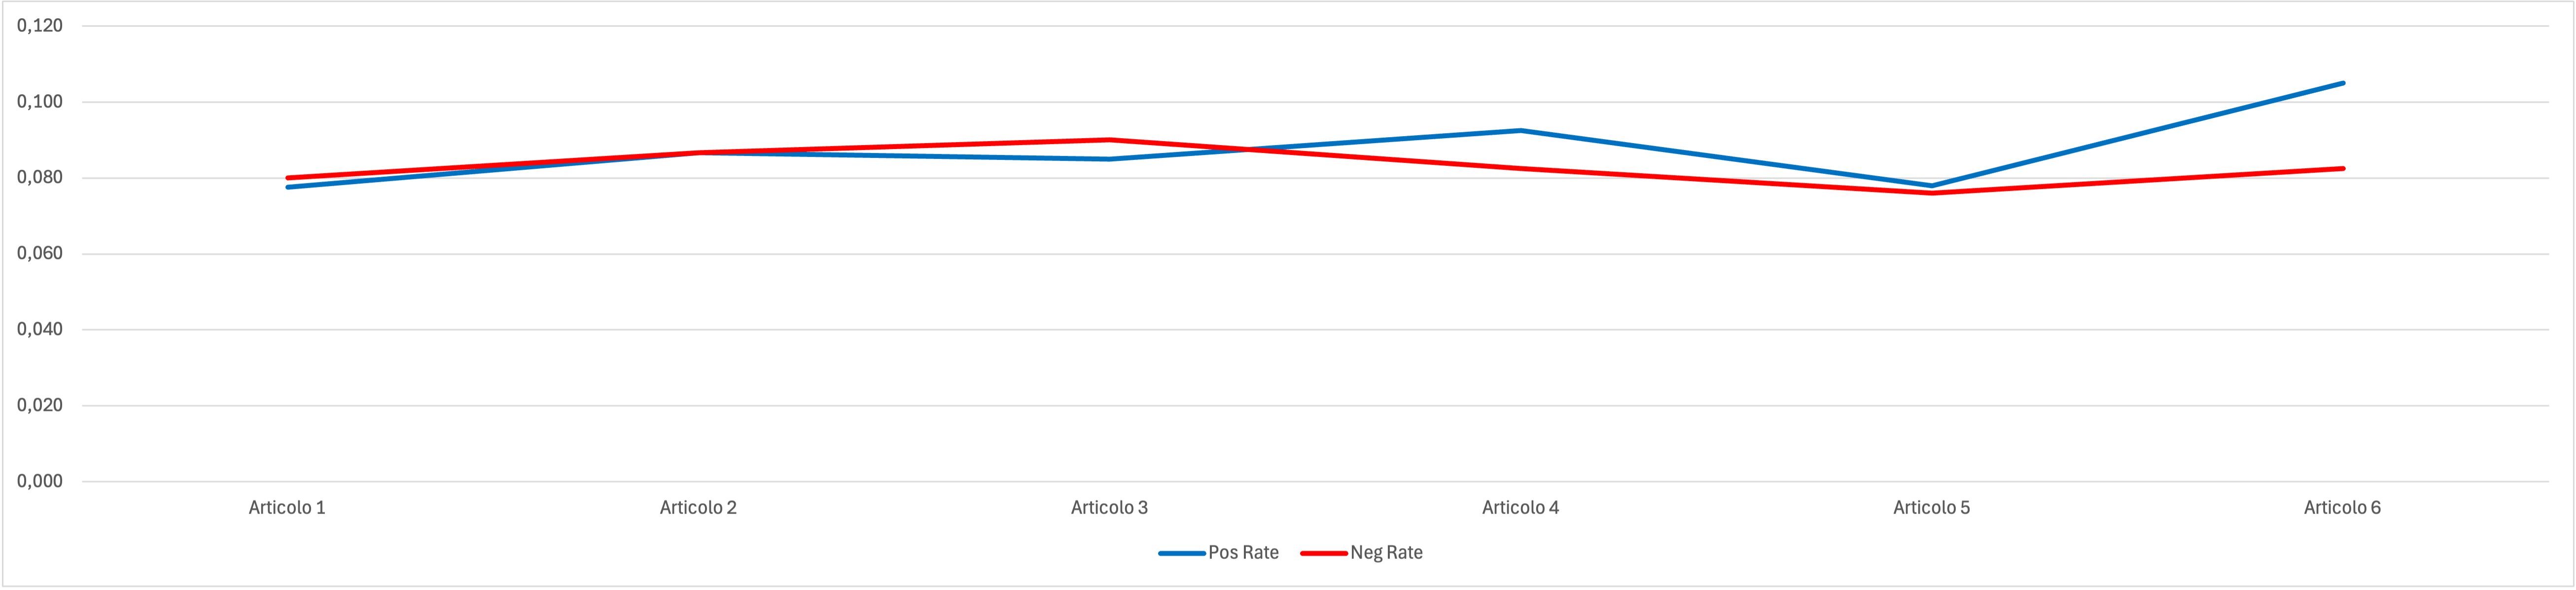
\includegraphics[width=1\linewidth]{Immagini/Neutrali/Neutrali- Sentiment Cronologico.png}
    \caption{Neutrali - Sentiment Cronologico.}
    \label{fig:enter-label-a5}

    \centering
    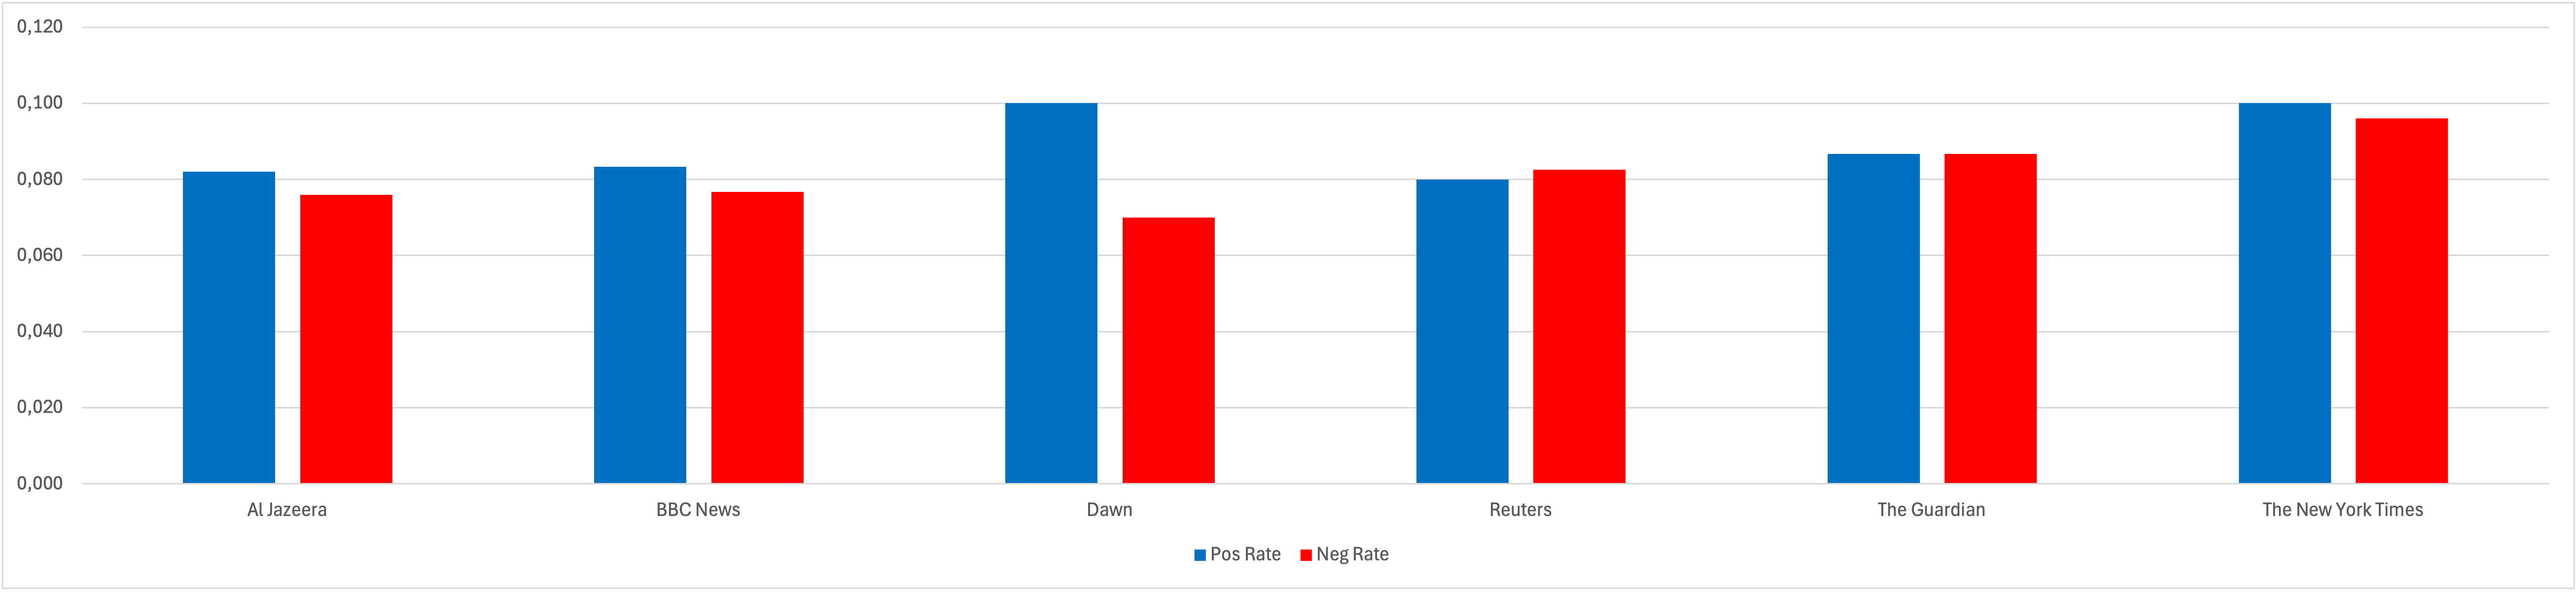
\includegraphics[width=1\linewidth]{Immagini/Neutrali/Neutrali- Sentiment Testate.png}
    \caption{Neutrali - Sentiment Testate.}
    \label{fig:enter-label-a5}
\end{figure}

\newpage
\subsection{Conservatori}

\begin{figure}[H]
    \centering
    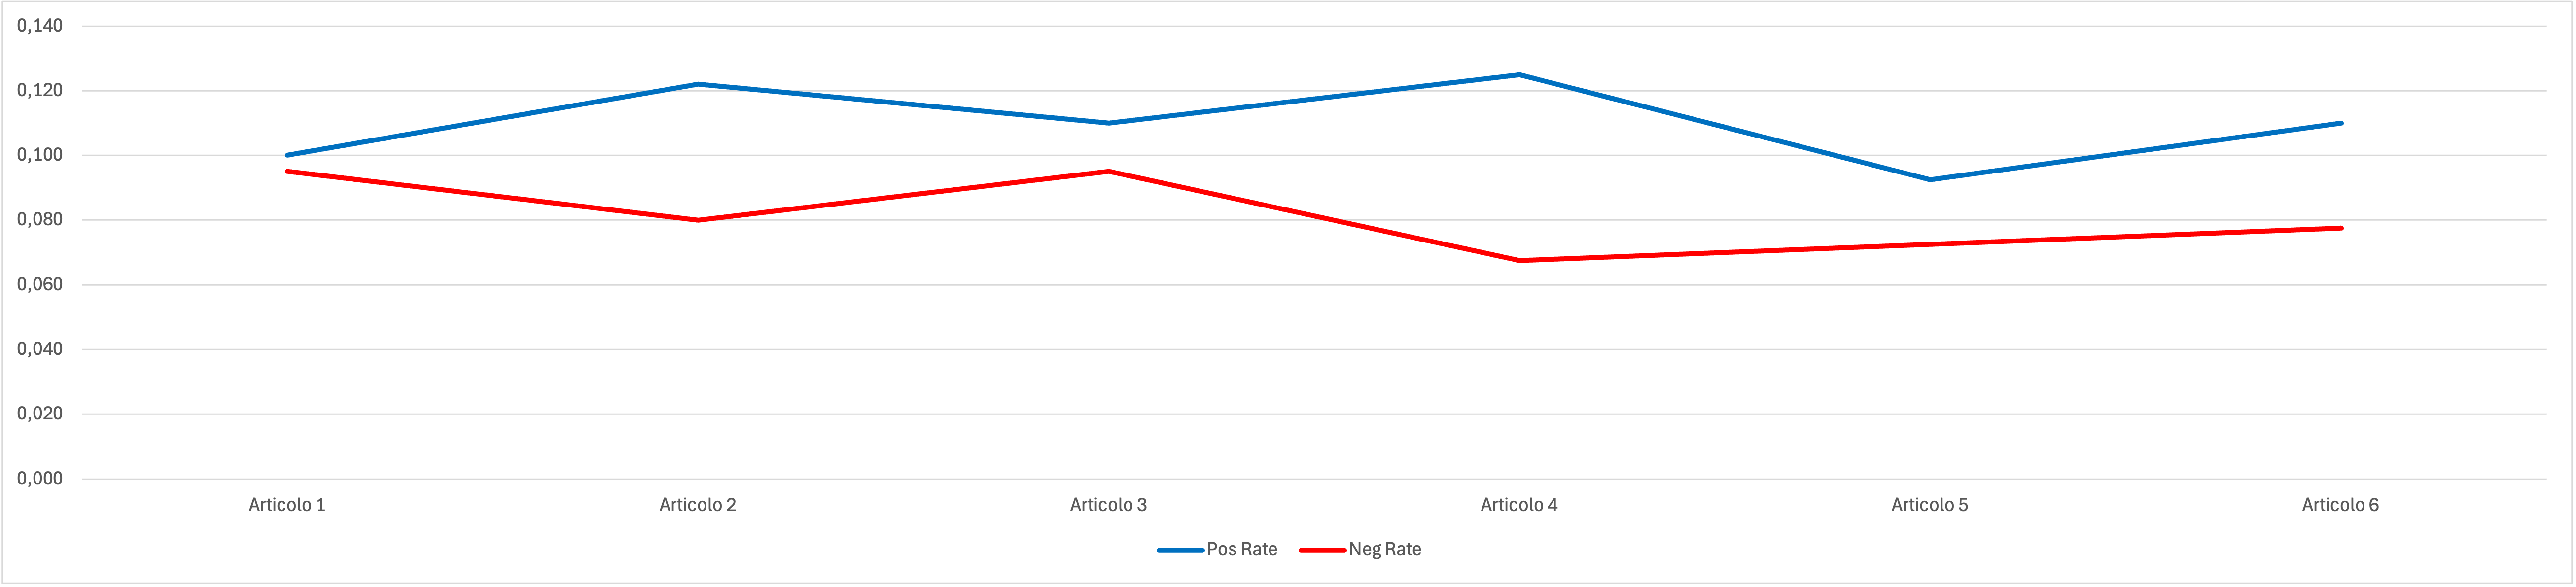
\includegraphics[width=1\linewidth]{Immagini/Conservatori/Conservatori - Sentiment Cronologico.png}
    \caption{Conservatori - Sentiment Cronologico.}
    \label{fig:enter-label-a5}

    \centering
    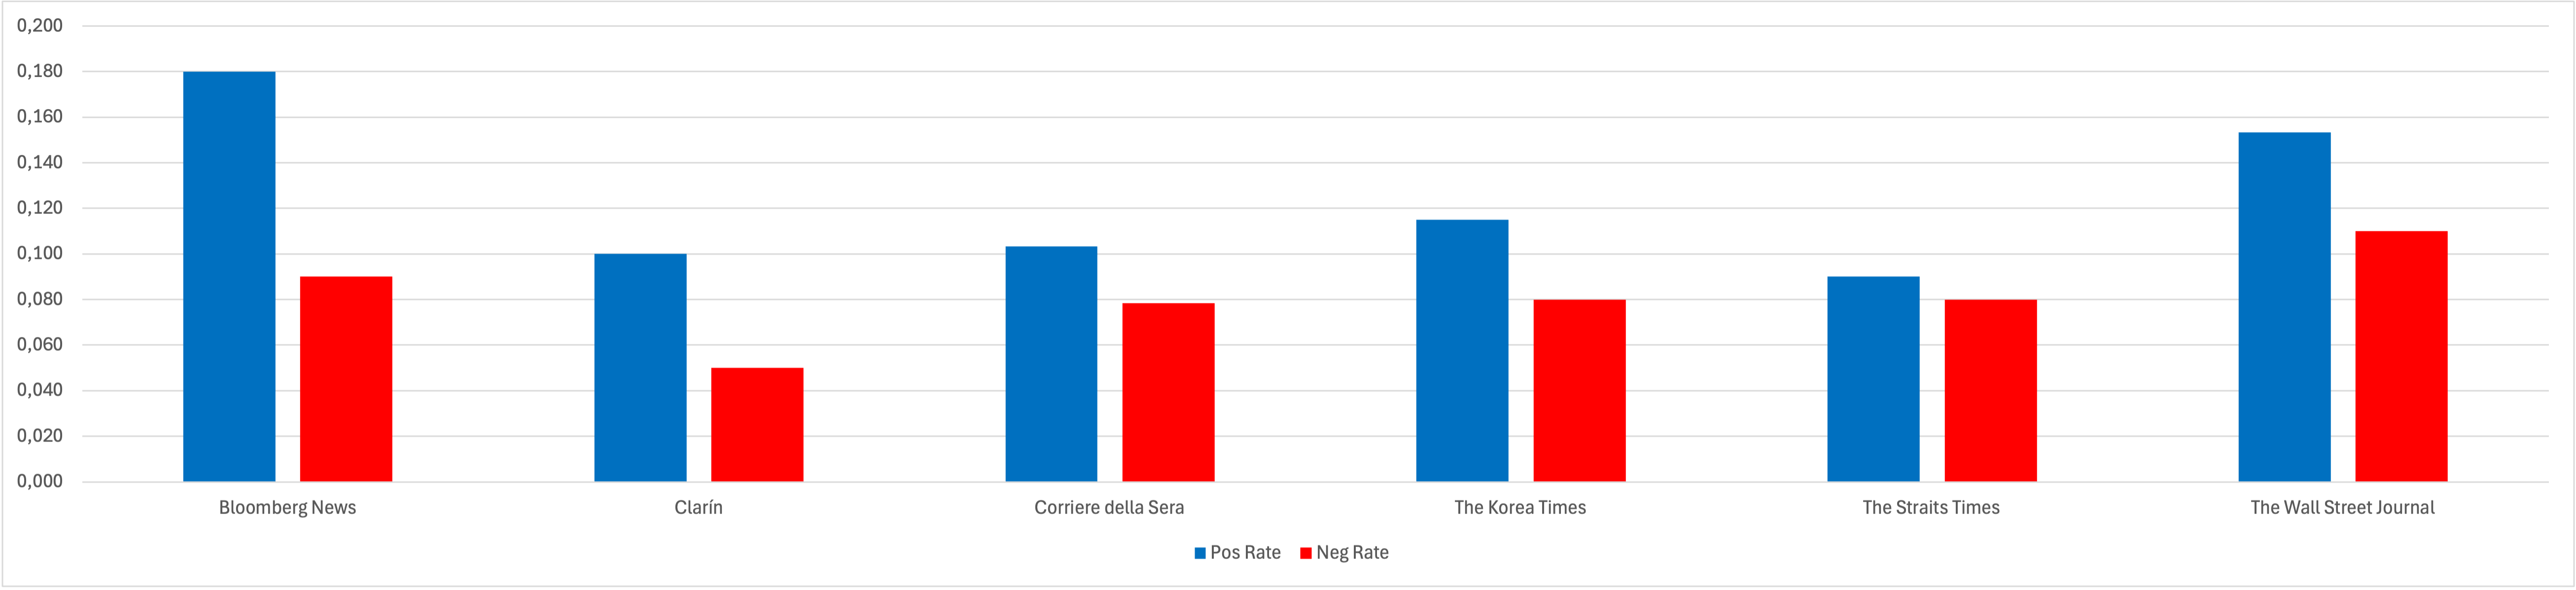
\includegraphics[width=1\linewidth]{Immagini/Conservatori/Cronologico - Sentiment Testate.png}
    \caption{Conservatori - Sentiment Testate.}
    \label{fig:enter-label-a5}
\end{figure}

\section{Statistiche di parole positive/negative}

\section{Sentiment aggregato e conclusioni}
    \chapter{Conclusioni e riflessioni finali}

\section{Implicazioni sul giornalismo politico}

\section{Limiti dello studio e sviluppi futuri}
    
    \cleardoublepage
    
    \printglossaries       % Stampa il glossario
    \printbibliography[heading=bibintoc] % Stampa bibliografia
\end{document}
